 \documentclass[a4paper,10pt]{article}
\usepackage[english]{babel}
\usepackage[utf8]{inputenc}
\usepackage[margin=1.5in]{geometry}
\usepackage{amsmath}
\usepackage{amsthm}
\usepackage{amsfonts}
\usepackage{amssymb}
\usepackage[usenames,dvipsnames]{xcolor}
\usepackage{graphicx}
\usepackage[siunitx]{circuitikz}
\usepackage{tikz}
\usepackage{hyperref}
\usepackage[numbers, square]{natbib}
\usepackage{fancybox}
\usepackage{epsfig}
\usepackage{soul}
\usepackage[framemethod=tikz]{mdframed}
\usepackage[shortlabels]{enumitem}
\usepackage[version=4]{mhchem}
\usepackage{fullpage}
\usepackage[nottoc, notlof, notlot]{tocbibind}
\setcounter{tocdepth}{2}

\def\hypothesis#1#2{{\color{purple}Hypothesis} {\color{blue}#1}: {\tt #2}}
\def\definition#1#2{{\color{purple}Definition} {\color{blue}#1} := {\tt #2}}
\def\ttt#1#2{{\tt{\color{black}#1} #2}}

%opening
\newtheorem{theorem}{Theorem}
\title{
\normalfont \normalsize 
\textsc{ENS Lyon} \\
[10pt] 
\rule{\linewidth}{0.5pt} \\[6pt] 
\huge Formalisation of the Delaunay Triangulation \\
\rule{\linewidth}{2pt}  \\[10pt]
}
\author{Clément Sartori}
\date{\normalsize 09/06/2017}

\begin{document}

\maketitle
\noindent
%Date Performed \dotfill December 31, 1999 \\
%Partners \dotfill Full Name \\
Advisor \dotfill Yves Bertot \\
%\title{Formalisation of the Delaunay triangulation}
%\author{Clément Sartori}


\maketitle

\begin{abstract}
  This report is the result of my internship at INRIA Sophia-Antipolis in the Marelle team, for the validation of the second year of my master's degree in Computer Science. During this internship I formalised Delaunay Triangulations in Coq. My code, although incomplete, can be found here: \href{https://github.com/Nemeras/StageDelaunay}{https://github.com/Nemeras/StageDelaunay}.
\end{abstract}

\tableofcontents{}

\newpage

\section{Introduction}
\rule{\linewidth}{0.5pt}

I did my second year of master's degree internship under the supervision of Yves Bertot at the INRIA Sophia-Antipolis in the Marelle team. 
The goal of this internship was to formalise the Delaunay triangulations in the {\sc{Coq}} proof assistant, that is, to try and find a minimal number of geometrical properties that had to be satisfied by sets of triangles in order for them to be Delaunay triangulations. One of the goal of the internship was to stay as close as possible to Knuth's paradigm in \cite{Knuth92} with CC systems (see Section \ref{CC}), by describing as many geometrical properties as possible using only combinatorial properties such as the orientation predicate ``is left of''.

\subsection{Triangulations and Applications}
Triangulations are a mathematical concept that is useful in a lot of domains. More particularly, Delaunay triangulation have quite a number of applications. For instance, they can be used to do shape morphing \cite{morphing}, or as their dual graph (the Voronoi diagram),  to modelise cellular coverage maps \cite{CelCov}, or for path planning \cite{PathPla}.

Since Delaunay triangulations are used in a lot of domains, a need of optimized algorithm and implementations of these algorithms has arised. For instance, the CGAL library \cite{cgal}, a software project aiming at providing access to efficient et reliable implementations of geometric algorithms provides a way to compute Delaunay triangulations \footnote{\href{http://doc.cgal.org/latest/Triangulation_2/index.html}{http://doc.cgal.org/latest/Triangulation$\_$2/index.html}}.

Moreover, because of their use, sometimes, in critical software, the need of proofs of the correctness of these algorithms and their implementations has arised. Jean-Francois Dufourd and Yves Bertot presented in \cite{Bertot} the first formalisation of the correctness of an algorithm to build a plane Delaunay Triangulation. Since Yves Bertot was my advisor during this internship, this work could be seen as trying to be the continuation of this previous work. However, in their work, they described triangles and other mathematical concept in a very ``low-level'' way, using complicated structures as hypermaps. On the contrary, this work tried to use a very ``high-level'', abstract point of view.

In geometry, a triangulation T of a subset X of $\mathbb{R}^d$ is a partition of this subset into simplices such that: 
\begin{itemize}
\item The intersection of two simplices is either empty or a face of those simplices.
\item Every bounded set of $\mathbb{R}^{d}$ cuts a finite number of simplices of T.
  \item The union of the simplices of T is X itself. \label{deftriangulation}
\end{itemize}

In the plane (where we stayed during this internship for simplicity's sake), the triangulation of a set of points is the partition of the convex hull of this set of points into triangles. Figure \ref{Trig1} is a triangulation while Figure \ref{NotTrig1} and \ref{NotTrig2} are not triangulations.
\begin{itemize}
\item In Figure \ref{NotTrig1}, the whole convex hull is not covered.
\item The Figure \ref{NotTrig2} isn't a partition.
 \end{itemize}

\begin{figure}
  \centering
  
  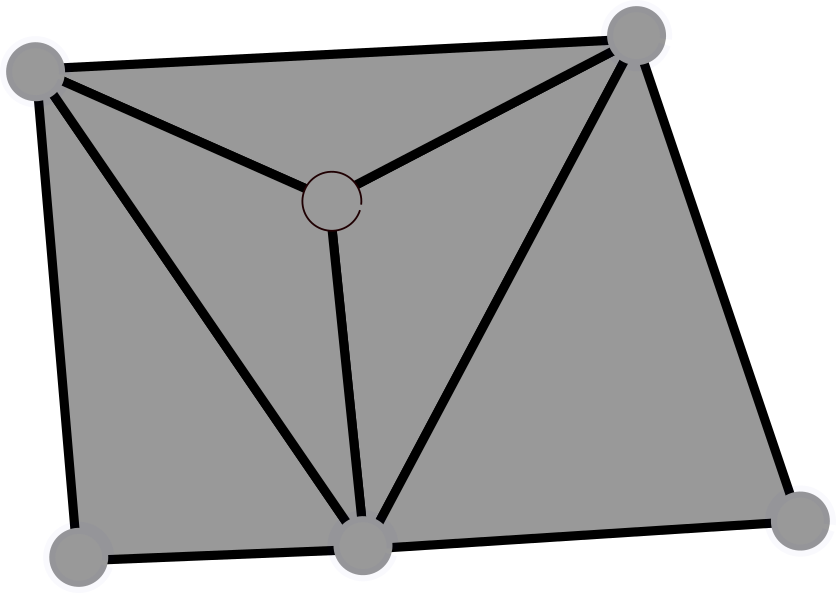
\includegraphics[scale=2]{Trig1}
  \caption{\label{Trig1} This is a triangulation}
\end{figure}

\begin{figure}
  \centering
  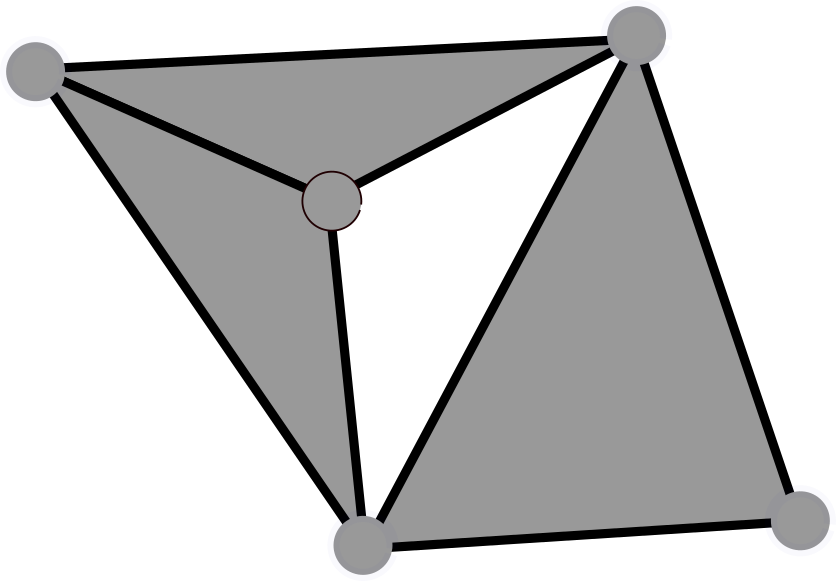
\includegraphics[scale=2]{NotTrig1}
  \caption{\label{NotTrig1} This is not a triangulation}
\end{figure}

\begin{figure}
  \centering
  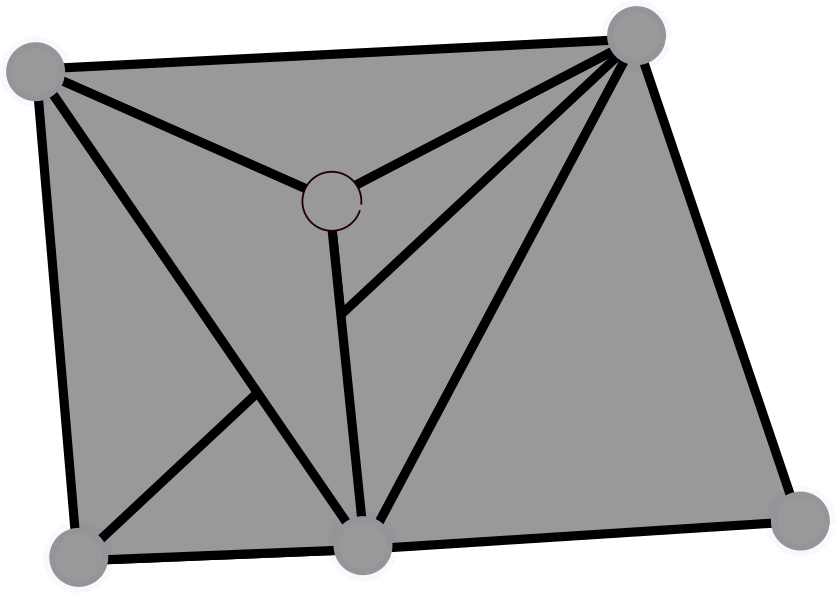
\includegraphics[scale=2]{NotTrig2}
  \caption{\label{NotTrig2} This is not a triangulation}
\end{figure}


More particularly, during this internship, we were interested in Delaunay triangulations: in the plane, a triangulation T of a set P of points is said to be a Delaunay triangulation if no point of P is in the circumcircle of a triangle of T. Figure \ref{notDelaunay} for instance, is not a Delaunay triangulation. Intuitively, a Delaunay triangulation is a triangulation that tries to maximise the smallest angle of any triangles, avoiding sliver triangles (triangles with one or two very acute angles).
\label{DelaunayCondition}
\begin{figure}
\centering
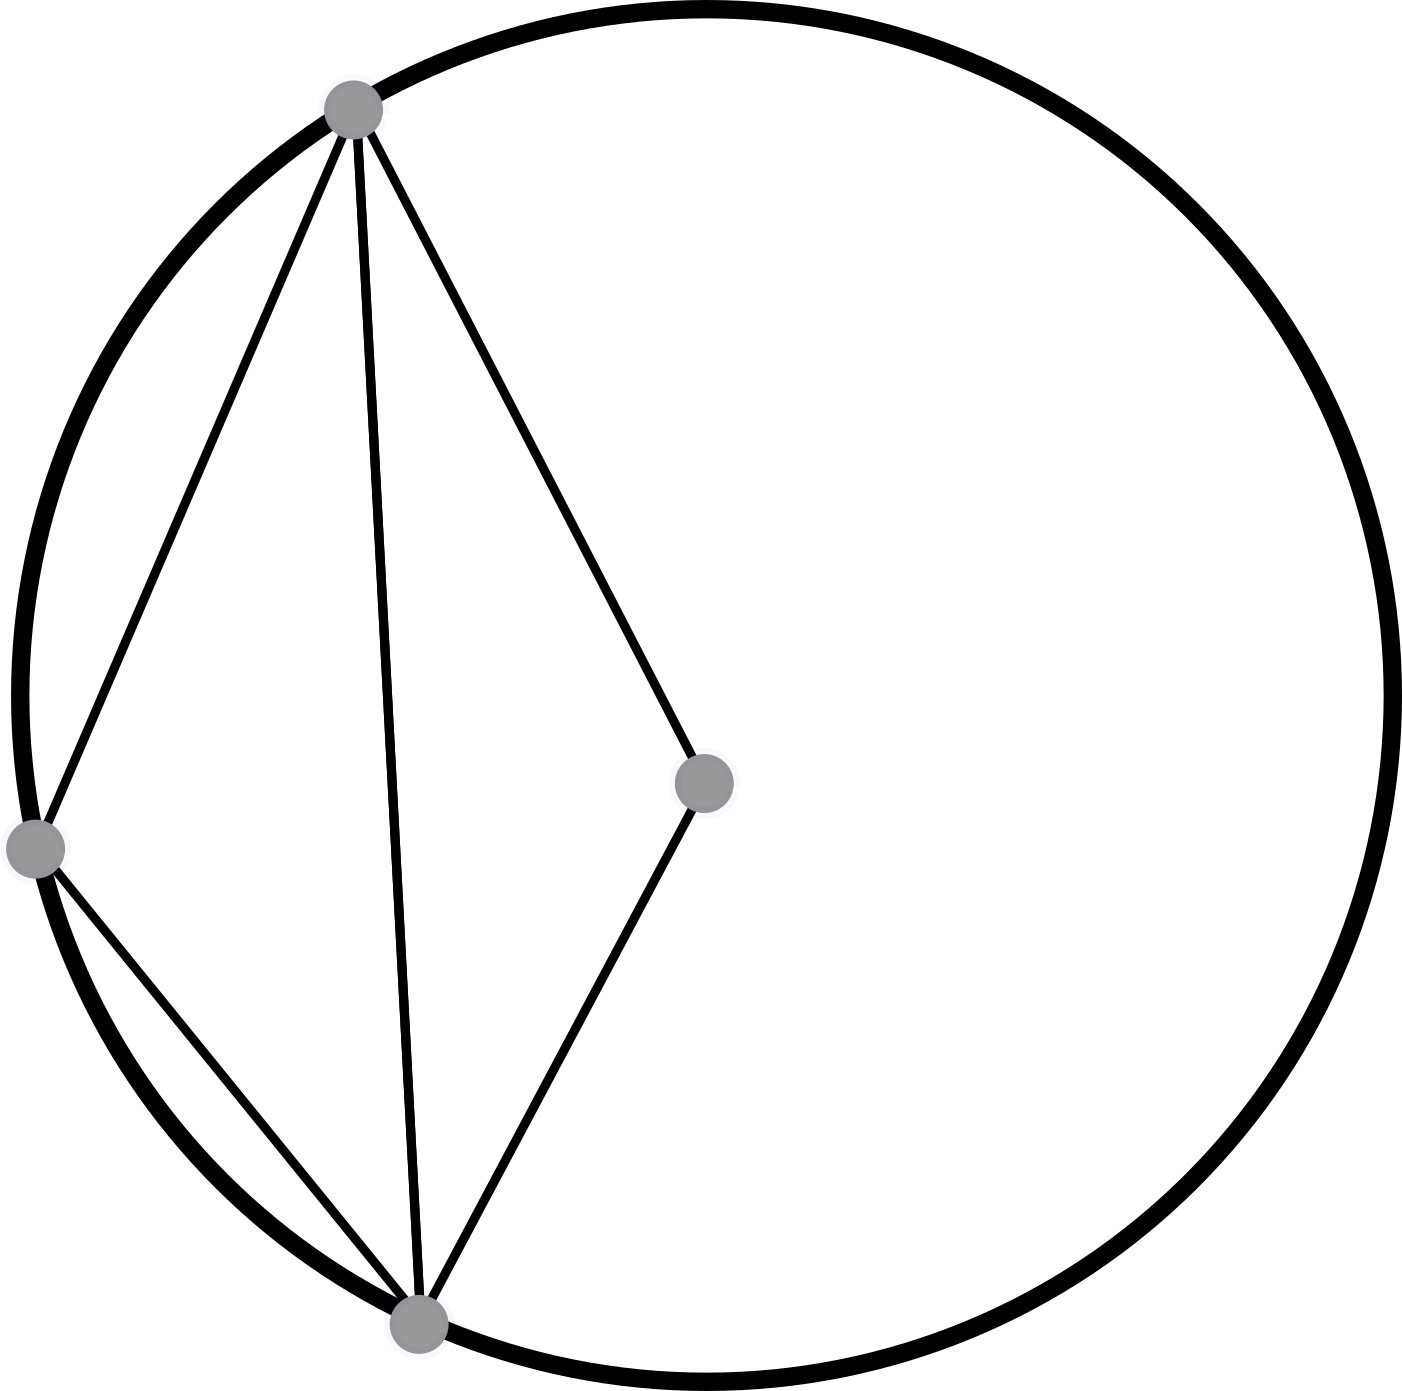
\includegraphics[scale=1]{dessin2}
\caption{\label{notDelaunay} Instance of a triangulation that is not a Delaunay triangulation}

\end{figure}


\subsection{Coq/The Mathematical Component library}

Machine-checked proofs are a research domain which is more than forty years (see \cite{Automath}) old. As such, the domain acquired a certain maturity; however, the main problem is the difficulty of use of proof assistants.

I wrote my formalisation of the Delaunay triangulation in the proof assistant {\sc Coq}, an environment in which one can express and prove mathematical assertions and which automatically checks the proofs you write in its language. The advantage of {\sc Coq} (and proof assistants in general) is that you can trust any {\sc Coq} proof as long as you trust {\sc Coq}'s kernel: {\sc Coq} totally relies on a part of its code, its ``kernel'', and this part of its code is intentionally kept small enough so it stays readable by a motivated reader. The choice of {\sc Coq} was very simple: {\sc Coq} is the most accomplished proof assistant, and has the enormous advantage of having access to the {\sc Mathematical Component} library.

To make proofs simpler, I used the {\sc{Mathematical Component}} library and the extension of {\sc{Coq}}'s tactic language, {\sc{SSReflect}}. The goal of the {\sc{Mathematical Component}} library project is to create a library of mathematical results, so that those result are easily reusable in {\sc{Coq}}. Examples of successful applications of the {\sc{Mathematical Component}} library and of {\sc{SSReflect}} are the proofs of the four-color theorem \cite{Gonthier08} and of the odd order theorem \cite{odd}. The four-color theorem states that it's possible to color any map with only four different colors, if we want to color any two adjacent regions with different colors. This result was conjectured in 1852 by Francis Guthrie. Some proofs were published, but they were false \cite{falseproof}. Finally, the solution was found in \cite{proof4} but the proof, for the first time, required a computer program, which made it quite disputed: now, the formalisation of \cite{Gonthier08} lets any computer check entirely the proof.

\subsection{CC Systems}
\label{CC}
CC (counter clockwise) Systems are a mathematical notions introduced by Donald Knuth \cite{Knuth92}. I's a ternary relation which is used to order triple of points $pqr$ in general position (no three points can be aligned) in the plane.

A CC system has to follow five axioms :
\begin{enumerate}
\item Cyclicity : $abc \rightarrow bca$.
\item Antisymmetry : $abc\rightarrow \neg bac$.
\item Nondegeneracy : $abc \vee bac$.
\item Interiority : $abd \rightarrow bcd \rightarrow adc \rightarrow abc$, see figure \ref{knuth4} later.
\item Transitivity : $ abc \rightarrow abd \rightarrow abq \rightarrow cbd \rightarrow dbq \rightarrow cbq $, see figure \ref{knuth5} later.
\end{enumerate}

A broader explanation of how we used Knuth's axioms here (without having the general position hypothesis) an be found in Section \ref{knuthpic}.


\section{The Algorithm}
\label{algo}
\rule{\linewidth}{0.5pt}

The goal of the internship was to study and prove the correctness of an algorithm to compute Delaunay triangulation. The context of the algorithm studied is, given a set of points in a plane, how to compute a Delaunay triangulation of the convex hull of this set of points. It is an incremental algorithm in two parts: given an existing triangulation and a point, the algorithm consists in:
\begin{enumerate}
\item adding the point to the existing triangulation to obtain a triangulation of the new set of points;
\item flipping the illegal edges to obtain a Delaunay triangulation.
\end{enumerate}

\subsection{Adding points}

In itself, adding the point to the existing triangulation is not a trivial problem, depending on whether the new point is in the convex hull of the existing points or not. In the litterature \cite{Del}, for incremental algorithms, it is generally considered that the points studied are inclosed within large triangles, which basically means that every new point will be in the convex hull of the previous ones. This was considered to be the case here. If this is not the case, then the problem of adding a new point which is not in the convex hull of the previous ones is equivalent to creating an incremental algorithm to compute the convex hull of a set of points. The formalisation of such an algorithm has been done by David Pichardie in \cite{Hull}.

Thus, adding a new point $P$ to a triangulation $T$, when $P$ is in the convex hull of the triangulation, is a two step process:
\begin{enumerate}
\item Finding the triangle $t$ of the triangulation in the interior of which $P$ is.
\item Replacing $t$ by three new triangles as in Figure \ref{adding}).
\end{enumerate}
\begin{figure}
\centering
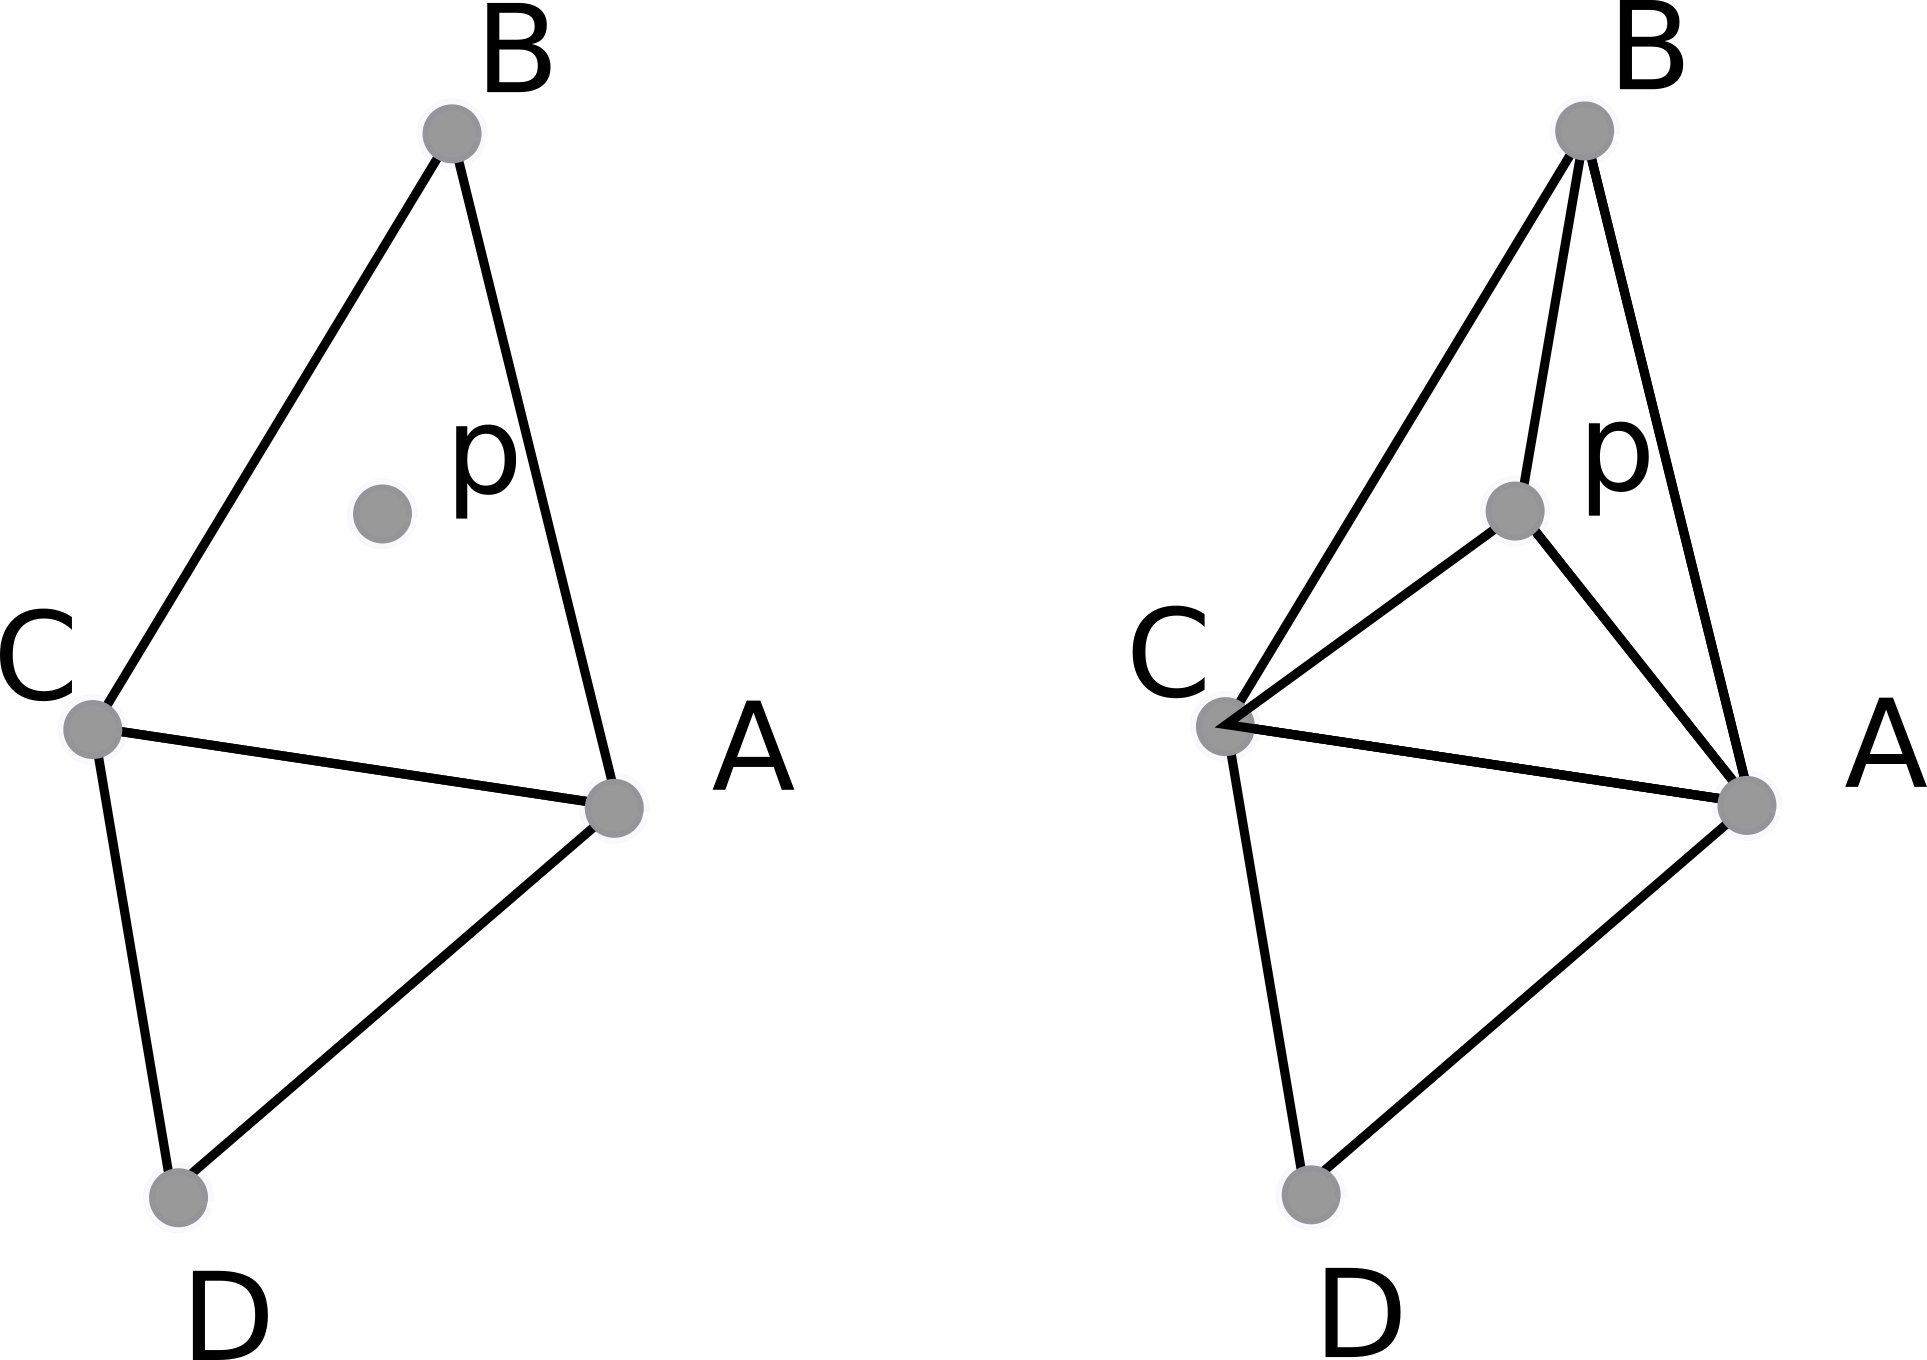
\includegraphics[scale=2]{adding}
\caption{\label{adding} Adding a point to a triangulation}
\end{figure}

It is worth noting that we do not treat the case where the new point is not in the interior of an existing triangle but is on the edge of one. There are multiples reasons for that. First, the subject of the internship was very vast: choices had to be made for which parts should be treated. Moreover, having a point on the the edge of a triangle would mean that three points of the data are aligned, and not ``having three aligned points'' is a very common hypothesis in computational geometry. 

There are multiple ways of finding the triangle in which P is. Since we are only interested in finite triangulations, one (naive) way is to just check every triangle to see if P is indeed in this triangle. The other (smarter and faster) way is to walk from triangle to triangle, selecting, each time, an edge separating this triangle from P, and carying on the search by going to the neighbouring triangle across from this edge. An example of this method, where we begin in the red triangle and try to find point P is described in Figure \ref{walk}.
The most naive approach was taken during this internship.

\begin{figure}
  \centering
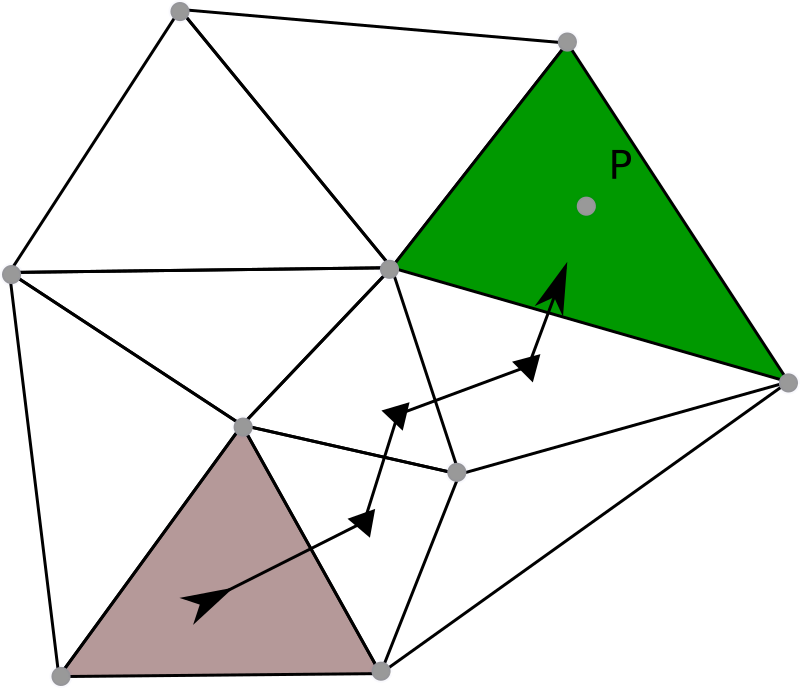
\includegraphics[scale=1]{Walk}
  \caption{\label{walk} Example of walk.}
\end{figure}


\subsection{Flipping edges}

It is possible, from any triangulation of a set of point, to obtain a Delaunay triangulation by repeating the same step: for each pair of triangles that does not meet the Delaunay condition (Section \ref{DelaunayCondition}), flip the common edge of the triangles.

For instance, while Figure \ref{notDelaunay} is not a Delaunay triangulation, the result of an edge-flipping step, Figure \ref{DelaunayTriangulation}, however, is a Delaunay triangulation
\begin{figure}
\centering

\includegraphics[scale=1]{dessin1}
\caption{\label{DelaunayTriangulation} Result of an edge-flipping step: example of Delaunay triangulation}
\end{figure}\\
This makes it possible to create a ``flipping'' algorithm: for any set of points, it is possible to obtain the Delaunay triangulation of this set of point by creating a random triangulation then applying this flipping step as many times as necessary.

As for the ``finding the triangle containing a particular point'' part, there are different possibilities : one can either check all triangles, at each step, to see if there is the need to flip some edges, or only check a subset of the triangles (those close enough to the new point of the triangulation). Again, we we only interested in the most naive approach during this internship.
\section{Formalisation of the Delaunay triangulation}
\rule{\linewidth}{0.5pt}

The goal of the formalisation is to stay as much as possible at a very abstract level, avoiding, for instance the use of complicated structures as hypermaps. Basically, the formalisation describes what properties every implementation of the concept should satisfy.

We describe in the sequel a formalisation of Delaunay triangulations. Any implementation should contain a type P for the points, a type T for the triangles, a type E for the edges, a type $\mathbb{R}$ for the coordinates of the points (a real integral domain where all elements are positive or negative), as well as some basic functions:
\begin{itemize}
\item A function \ttt{vertices\_to\_edge}{} to create an edge from two points.
\item A function \ttt{vertices\_to\_triangles}{} to create a triangle from three points.
\item A function \ttt{vertex}{}  that should be able to return the first, second or third vertex of a triangle.
\item A function \ttt{xCoord}{} that returns the X coordinate of a point.
\item A function \ttt{yCoord}{} that returns the Y coordinate of a point.
\end{itemize}

For {\tt vertices\_to\_edge} and {\tt vertices\_to\_triangle}, two different choices were made:
for all {\tt a}, {\tt b}, {\tt c}, {\tt vertices\_to\_edge a b} and {\tt vertices\_to\_edge b a} create the same edge, whereas {\tt vertices\_to\_triangle a b c} and {\tt vertices\_to\_triangle c a b} create different triangles. Indeed, a lemma was needed to get simpler proofs; this lemma states that, as long as {\tt a}, {\tt b} and {\tt c} form a well-oriented triangle, then the first vertex of {\tt vertices\_to\_triangle a b c} will be {\tt a}, the second one will be {\tt b} and the last one {\tt c}. This added a condition on the implementation of triangles : for {\sc Coq}, the triangle {\tt abc} should not be equal to the triangle {\tt bca}. Even if can seem counter-intuitive, it was the most practical choice. 


\subsection{Geometrical predicates}
\label{predicate}
Any implementation should also contain some geometrical predicates:
\begin{enumerate}
\item \ttt{is\_left\_or\_on\_line}{$a$ $b$ $c$} and \ttt{is\_left\_of}{} which test if the point $c$ is (strictly) left of the points $a$,$b$ e.g. if $a$,$b$,$c$ form a (strictly) well-oriented (counter-clockwise) triangle.
\item \ttt{in\_circle}{$p$ $a$ $b$ $c$} which tests if a point $p$ is in the circumcircle of the triangle described by $a$,$b$,$c$.
\item \ttt{in\_triangle\_w\_edges}{$t$ $p$} and \ttt{in\_triangle}{$t$ $p$} which test if $p$ is (strictly) in $t$.
  \item \ttt{is\_on\_line}{} which tests is 3 points are aligned.

\end{enumerate}

Those predicates are derived from another function, which is required in any implementation: \ttt{oriented\_surface}{$a$ $b$ $c$}, computing the oriented surface described by the three points $a$,$b$,$c$:
\begin{itemize}
\item \ttt{is\_left\_of}{a b c = oriented\_surface a b c > 0}
  \item \ttt{is\_left\_or\_on\_line}{a b c = oriented\_surface a b c $\geq$ 0}
  \item \ttt{is\_on\_line}{a b c = oriented\_surface a b c = 0}
 \item \ttt{oriented\_triangle}{t = oriented\_surface (vertex1 t) (vertex2 t) (vertex3 t) $\geq$ 0} 
  \end{itemize}.


  {\tt oriented\_surface a b c} is the oriented surface (see Figure \ref{surface}) of the triangle {\tt abc}. It is non-negative if {\tt abc} is oriented counter-clockwise , nonpositive otherwise (and null if {\tt a b} and {\tt c} are aligned).
Usually, it is computed from a determinant, as seen in the implementation presented in Section \ref{implementation}. Thus, the hypotheses from Section \ref{Hypothesis} feel safe.

\begin{figure}
  \centering
  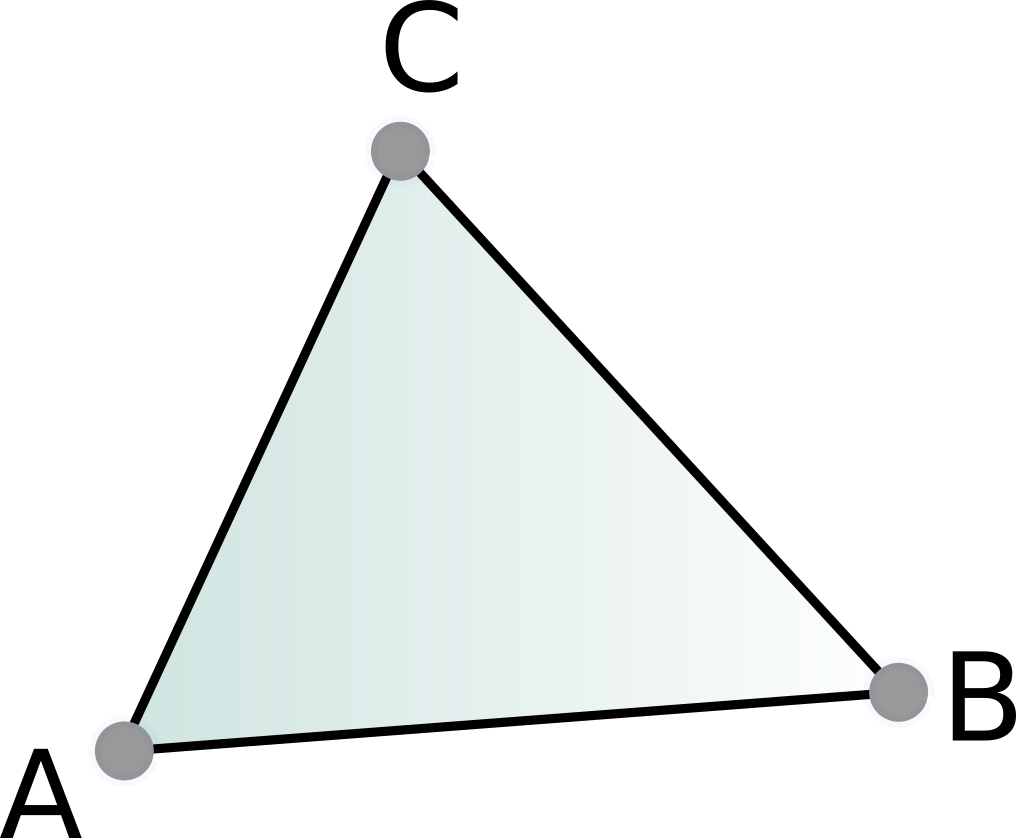
\includegraphics{Surface}
  \caption{\label{surface} Here, ABC has a positive oriented surface whereas ACB has a negative oriented surface.}
\end{figure}


  The predicate \ttt{is\_left\_of}{} is inspired by Knuth's idea of CC systems \cite{Knuth92}.
  However, unlike him, we do not consider that our points are in general position (we recall that points are considered in general positions if no three points are aligned): the oriented surface of three points can then be 0. Thus, the opposite of \ttt{is\_left\_of}{a b c} is not \ttt{is\_left\_of}{b a c} but \ttt{is\_left\_or\_on\_line}{b a c}. A broader explanation of what happens to Knuth's axioms when degenerate cases (aligned points) exist can be found in \cite{Hull}. \label{knuthpic}

  Then, from those predicates, we can define what means to be in a triangle :
  \begin{itemize}
    \item \begin{tabular}{ll}
       \ttt {in\_triangle}{t p = }& \ttt{}{is\_left\_of (vertex1 t) (vertex2 t) p} $\wedge$\\
        &\ttt{}{is\_left\_of p (vertex2 t) (vertex3 t)} $\wedge$\\
  & \ttt{}{is\_left\_of (vertex1 t) p (vertex3 t)}
      \end{tabular}
\item \begin{tabular}{ll}
       \ttt{in\_triangle\_w\_edges t p}{= }& \ttt{}{is\_left\_or\_on\_line (vertex1 t) (vertex2 t) p} $\wedge$\\
        & \ttt{}{is\_left\_or\_on\_line p  (vertex2 t) (vertex3 t)} $\wedge$\\
  & \ttt{}{is\_left\_or\_on\_line (vertex1 t) p (vertex3 t)}
      \end{tabular}
      \end{itemize}

  \subsection{Hypotheses}
\label{Hypothesis}
We put assumptions (which have to be proven when doing an implementation) on the implementations of the predicates/functions. The following ones are simple:
\begin{itemize}
\item \hypothesis{oriented\_surface\_xx}{$\forall$ x y, {\tt oriented\_surface x x y} = 0}.
  
  The oriented surface of a segment is 0.
\item \hypothesis{oriented\_surface\_circular}{$\forall$ a b c, oriented\_surface a b c = oriented\_surface c a b}.
  
  The oriented surface of {\tt abc} is the same as the one of {\tt cab}, because we don't change the order of the points.
\item \hypothesis{oriented\_surface\_change}{$\forall$ a b c, oriented\_surface a b c = - oriented\_surface b a c}.
  
  The oriented surface of {\tt abc} is the same as the one of {\tt bac}, because we change the order of the points.
\item \hypothesis{vertices\_to\_edge\_sym}{$\forall$ a b, vertices\_to\_edge a b = vertices\_to\_edge b a}.

  Edges don't care about the order of their vertices.
  \item 
    \hypothesis{vertices\_to\_triangle\_oriented}{$\forall$ a b c, oriented\_triangle (vertices\_to\_triangle a b c).}

    {\tt vertices\_to\_triangle} always return an oriented triangle, thus sometimes changing the order of the points to do it.
\item\hypothesis{is\_on\_line\_trans}{$\forall$ a b c d, a != b $\rightarrow$ is\_on\_line a b c $\rightarrow$ is\_on\_line a b d $\rightarrow$
    is\_on\_line a c d}.
  
  if {\tt a}, {\tt b} and {\tt c} are aligned, {\tt a} and {\tt b} are different and {\tt a} {\tt b} and {\tt d} are aligned, then {\tt a} {\tt c} and {\tt d} are aligned (see Figure \ref{aligned}).

  \begin{figure}
    \centering
    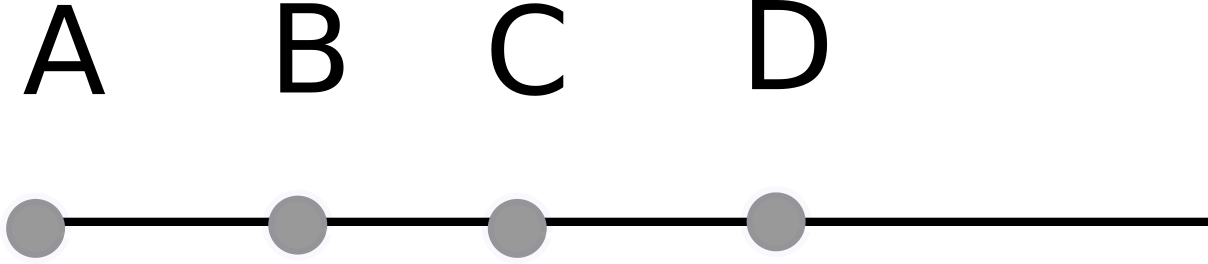
\includegraphics{aligned}
    \caption{\label{aligned} Four aligned points}
  \end{figure}
  
\item \hypothesis{vertices\_to\_triangle\_correct2}{\\$\forall$ a b c, $\forall$ t,
          (t = vertices\_to\_triangle a b c) $\rightarrow$\\
          ((a $\in$ vertex\_set t) $\wedge$ (b $\in$ vertex\_set t) $\wedge$ (c $\in$ vertex\_set t))}.
        
        {\tt a}, {\tt b} and {\tt c} should be vertices of {\tt vertices\_to\_triangle a b c}.


      \item \hypothesis{vertices\_to\_triangle\_correct}{$\forall$ a b c, 
    is\_left\_or\_on\_line a b c $\rightarrow$\\
    a = vertex1 (vertices\_to\_triangle a b c) $\wedge$\\
    b = vertex2 (vertices\_to\_triangle a b c) $\wedge$\\
    c = vertex3 (vertices\_to\_triangle a b c).}

  If {\tt a}, {\tt b} and {\tt c} form a strictly well-oriented triangle, then the first vertex of {\tt vertices\_to\_triangle a b c} should be {\tt a}, the second one should be {\tt b} and the last one {\tt c}.

        

\end{itemize}
There are also assumptions on the functions that are made to link functions between each other: for instance, to explain what is the edge set of a strictly well-oriented triangle created thanks to vertices-to-triangle:

\hypothesis{edges\_set\_vertices\_to\_triangle:}
  {\\$\forall$ a b c, is\_left\_of a b c $\rightarrow$
    edges\_set (vertices\_to\_triangle a b c) =\\ 
                       $[$ fset (vertices\_to\_edge a b);
                           (vertices\_to\_edge a c);
                           (vertices\_to\_edge b c) $]$}.

                         "The edge set of a triangle created with {\tt vertices\_to\_triangle a b c} should be the set containing the edge {\tt ab}, the edge {\tt ac} and the edge {\tt bc}.
                         
Some assumptions are harder, because they are generalizations of Knuth's axioms or just come from more elaborated geometrical facts. For instance:
\begin{itemize}
\item \hypothesis{is\_left\_of\_trans}{(Figure \ref{knuth5}):\\  \begin{tabular}{lll}
                                          $\forall$ a b c d q, &is\_left\_of a b c $\rightarrow$\\
                                           &is\_left\_of a b d $\rightarrow$\\
                                           &is\_left\_of a b q $\rightarrow$\\
                                           &is\_left\_of q b d $\rightarrow$\\
                                           &is\_left\_of d b c $\rightarrow$\\
                                           &is\_left\_of q b c 
           \end{tabular} }.
\\
\begin{figure}
\centering
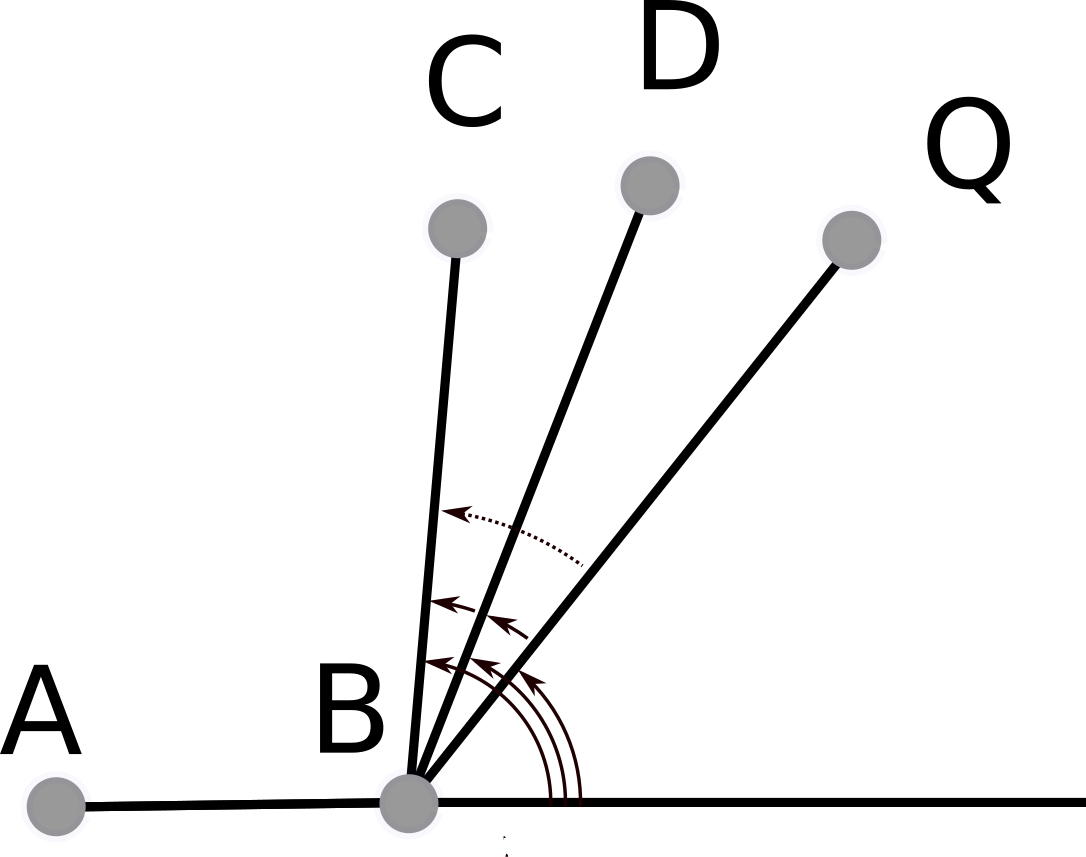
\includegraphics[scale=2]{Axiom5}
\caption{\label{knuth5} Knuth's 5$^{th}$ Axiom}
\end{figure}\\
The idea to understand this hypothesis is that it sorts {\tt c d} and {\tt q} in a semi-plane defined by {\tt a} and {\tt b}.
\item \hypothesis{Axiom 4}{(Figure \ref{knuth4}):\\ \begin{tabular}{ll}
             $\forall$ a b c d,                  &is\_left\_of a b d $\rightarrow$\\
                                           &is\_left\_of b c d $\rightarrow$\\
                                           &is\_left\_of c a d $\rightarrow$\\
                                           &is\_left\_of a b c
           \end{tabular}}.
\begin{figure}
\centering
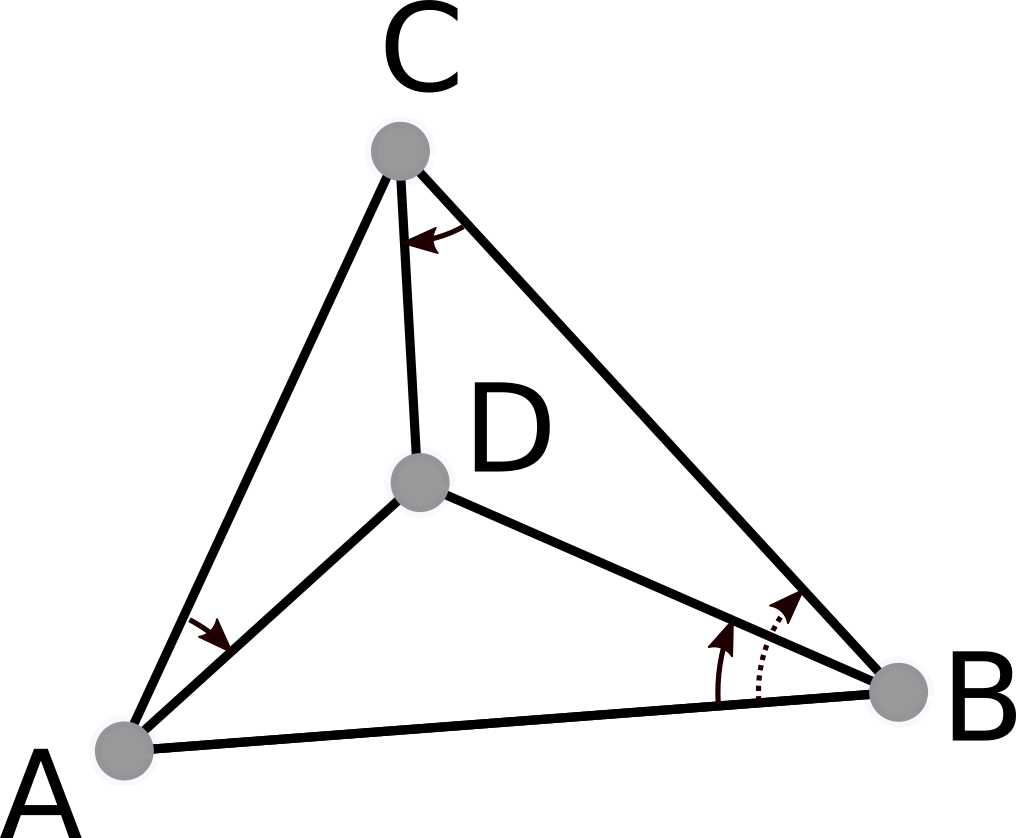
\includegraphics[scale=2]{Axiom4}
\caption{\label{knuth4} Knuth's 4$^{th}$ Axiom}
\end{figure}\\
\item \hypothesis{on\_line\_on\_edge}{(Figure \ref{edge_line}):\\
  $\forall$ a b c, is\_left\_of a b c $\rightarrow$ $\forall$ q, is\_on\_line a c q $\rightarrow$ 
                                   is\_left\_of a b q $\rightarrow$\\ is\_left\_of b c q $\rightarrow$
                                   on\_edge (vertices\_to\_edge a c) q.}
\\
\begin{figure}
\centering

\includegraphics[scale=2]{oloe}
\caption{\label{edge_line} Link between the geometrical predicates and being on an edge}
\end{figure}
\item \hypothesis{on\_edge\_on\_line}{(Figure \ref{edge_line}):\\
  $\forall$ a b c, is\_left\_of a b c $\rightarrow$
  $\forall$ q, on\_edge (vertices\_to\_edge a c) q $\rightarrow$ \\
           is\_on\_line a c q $\wedge$ is\_left\_of a b q $\wedge$ is\_left\_of b c q.}

         This hypothesis and the next one are here to create a link between the geometrical predicates such as {\tt is\_left\_of} and fact that a point is (or not) on an edge.
       \item \hypothesis{intersection\_of\_lines}{(Figure \ref{intersection_line}):
            $\forall$ a b c d,
is\_left\_of a b c -> is\_on\_line a b d ->
is\_on\_line a c d -> d = a.}
\\\begin{figure}
\centering
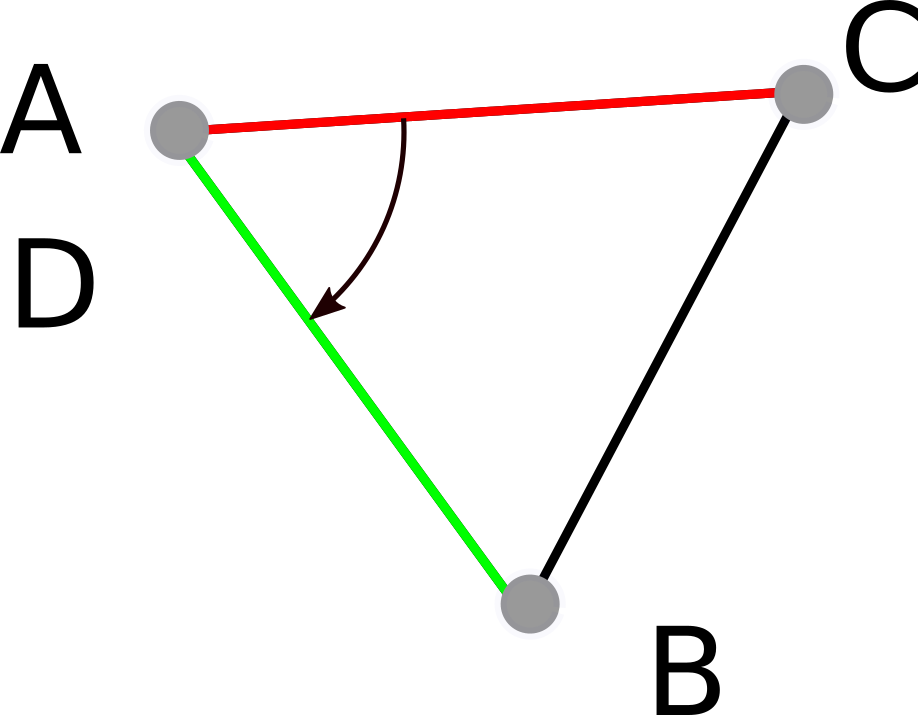
\includegraphics[scale=2]{il}
\caption{\label{intersection_line} The intersection of two lines that are not parallel is a point !}
\end{figure}
\end{itemize}



\subsection{Geometrical Properties}
\label{definition_triangulation}
We define a triangulation Tr on a data set D as a finite set of triangles with points of D as vertices which satisfies some properties:
\begin{enumerate}
\item \ttt{covers\_hull}{Tr D}: the whole convex hull of D is covered by the triangles of Tr.
\item \ttt{covers\_vertices}{Tr D}: the points of D are exactly the vertices of the triangle of Tr.
\item \ttt{no\_cover\_intersection}{} Figure \ref{nci}: there is no point which is in the interior of two different triangles of the triangulation . This is expressed as enforcing that if two triangles of the triangulation have a common interior point, then the two triangles are actually the same.
  \item\ttt{no\_point\_on\_segment}{} Figure \ref{nps}: no point can be simultaneously a vertex of a triangle, and on the edge of another triangle (remark: the vertex of a triangle is considered to not be on the edge of this triangle). This is written as: if a vertex $P$ of a triangle $t$ of the triangulation is in another triangle $t'$ of the triangulation, then $P$ is a vertex of $t'$.
\item \ttt{triangle\_3\_vertices}{Tr}: every triangle of the triangulation has 3 vertices.
\item \ttt{triangle\_nempty}{Tr}: no triangle of {\tt Tr} is empty (no flat triangle).
\item \ttt{oriented\_triangle\_triangulation}{Tr}: all triangles of the triangulation are strictly well-oriented.

  Remark: by hypothesis, we force \ttt{vertices\_to\_triangle}{} to return a well-oriented triangle so this hypothesis is quite simple to prove in general.
\end{enumerate}
The first two properties express that the finite set of triangles Tr is indeed a triangulation of the whole data set D, and covers its convex hull with triangles, in order to respect the third part of the definition of a triangulation (see Section \ref{deftriangulation}).
Then, the next two properties are here to avoid problems with how the triangles are positioned: 
\begin{enumerate}
\item \ttt{no\_cover\_intersection}{} is here to avoid problems like in Figure \ref{nci} where two triangles {\tt ABC} and {\tt DEF} aren't well positioned; there exists a point {\tt P} that is both in the interior of {\tt ABC} and {\tt DEF}.
\\
\begin{figure}
\centering
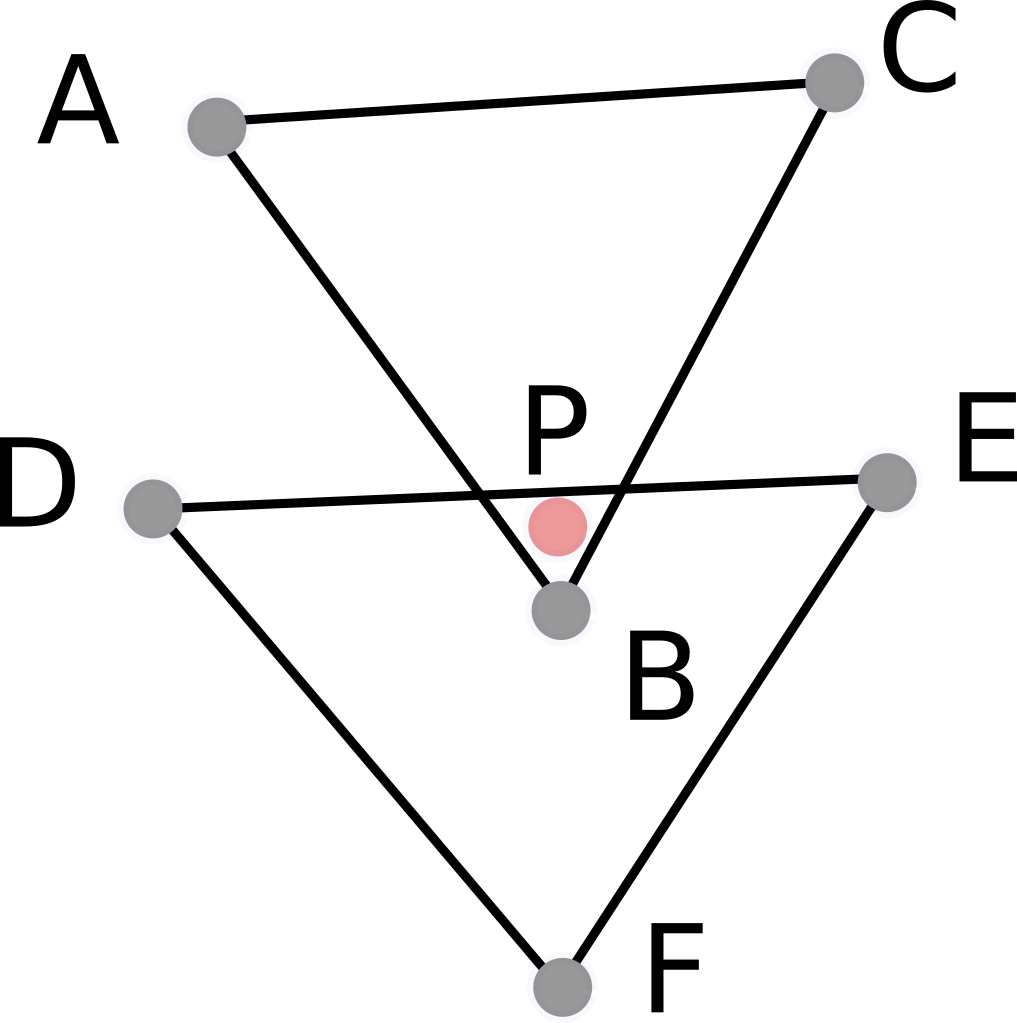
\includegraphics[scale=2]{nci}
\caption{\label{nci} {\tt no\_cover\_intersection}}
\end{figure}
\item \ttt{no\_point\_on\_segment}{} is here to avoid problems like in Figure \ref{nps}, where the vertice {\tt B} of the triangle {\tt ABC} is on the edge {\tt DE} of the triangle {\tt DEF}.
\\
\begin{figure}
\centering
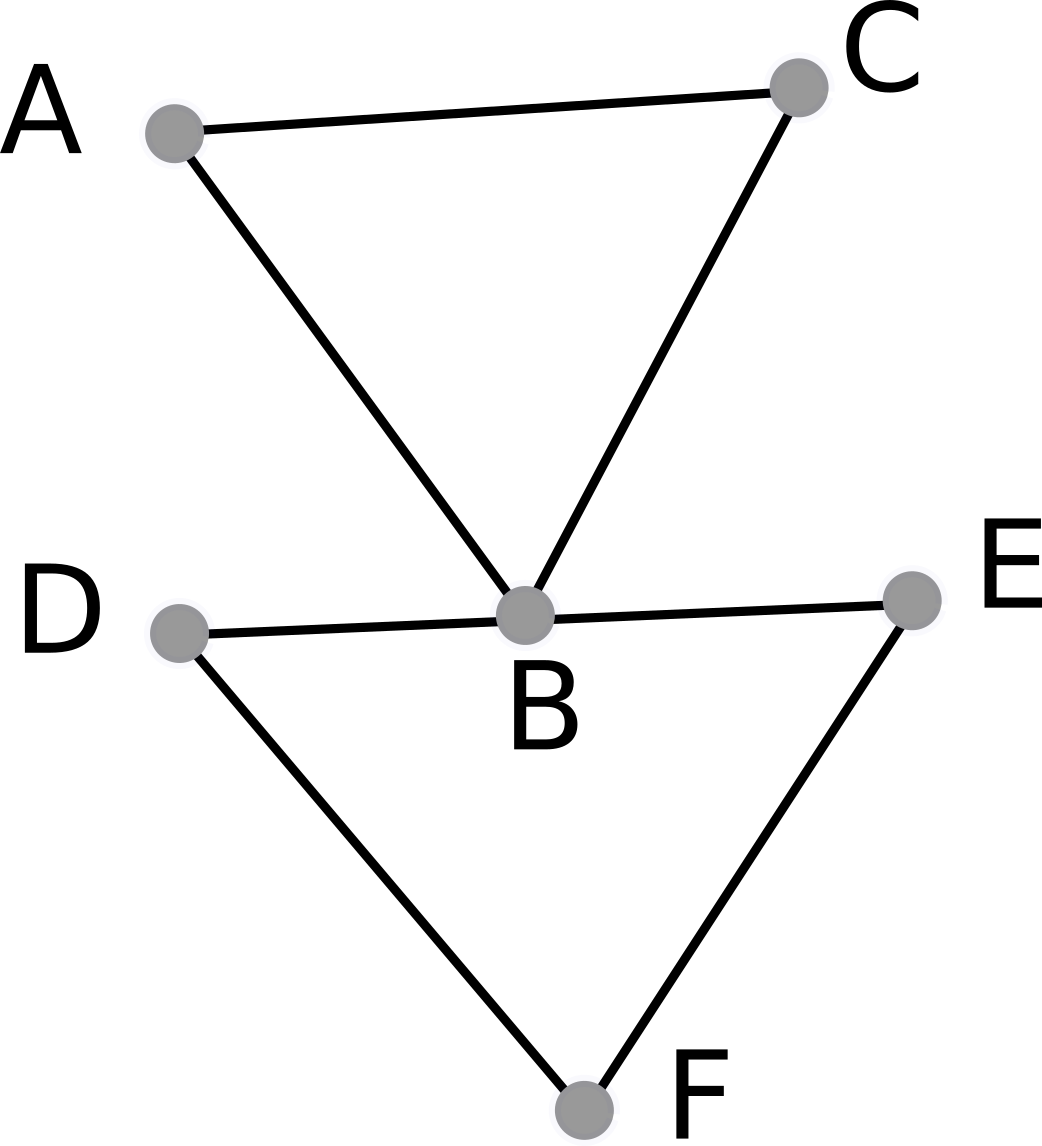
\includegraphics[scale=2]{nps}
\caption{\label{nps} {\tt no\_point\_on\_segment}}
\end{figure}
\end{enumerate}
In both case, the properties are here to ensure that the first part of the definition of a triangulation is respected: the intersection of two simplices should either be empty or a face of those simplices.

The last three properties are here to avoid degenerate cases with the triangles of the triangulation (triangulation should not contain degenerate triangles). It is to be noted that the third property should imply the second one, which implies the first one. However, the proof of this is not trivial, and I had to add those properties late during the internship, which means I did not have the time to do them.

\subsection{Convex Hulls}

The definition of what a triangulation is in dimension 2 requires first to define what a convex hull of a point set D is.
There are two different approaches:
\begin{enumerate}
\item The first possibility, used by Knuth,  is to define the convex hull as a cyclic sequence S: {\tt (S1; S2; ...; Sn; S1)} of elements of D such that every point of D is ``encompassed'' within S, with {\tt P} being ``encompassed'' within S if and only if, for all i,  {\tt is\_left\_or\_on\_line Si Si+1 P} is true.

\item The second possibility is via the notion of barycenter: it is the smallest convex set {\tt H} such that every point of {\tt H} is a barycenter for any choice of positive weight of the points of {\tt D}.
\end{enumerate}

It is the second approach that we used in our formalisation. It has two main benefits:
\begin{enumerate}
\item First, it is independent of the dimension, whereas the first possibility only works in dimension 2.
\item It is independent of the definition of the geometrical predicates, and those can change (for instance between Knuth's case where points are in general positions and cases where they are not). 
\end{enumerate}
Also, it is very nicely linked to {\tt oriented\_surface} in dimension 2. Carathéodory's theorem for convex hulls indicates the following:
\begin{theorem}
If a point of $\mathbb{R}^d$ lies in the convex hull of {\tt D}, then it is a barycenter of $d+1$ points of {\tt D}.
\end{theorem}
In dimension 2, this means that every point in the convex hull of {\tt D} is a barycenter of three points of {\tt D} (ie, in a triangle with vertices some points of {\tt D}).
Moreover, there is a nice property about the barycentric coefficients: if $x$ is in $ABC$ then we have:
$$x = x_AA + x_BB + x_CC$$
with: $x_A =\frac{ \text{\tt oriented\_surface B C x}}{\text{\tt oriented\_surface A B C}}$,
$x_B =\frac{ \text{\tt oriented\_surface C A x}}{\text{\tt oriented\_surface A B C}}$ and
$x_C =\frac{ \text{\tt oriented\_surface A B x}}{\text{\tt oriented\_surface A B C}}$
, which gives an elegant relation between the coefficients and the surface of the triangles (Figure \ref{cara}).

\begin{figure}
  \centering
  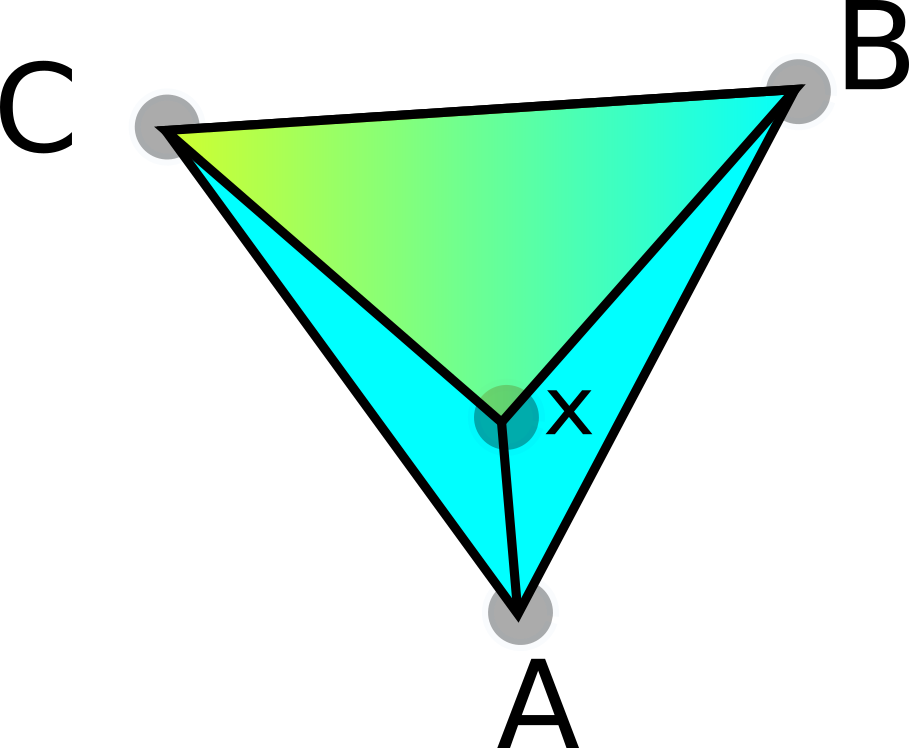
\includegraphics[scale=2]{cara.png}

  \caption{\label{cara} Relation between barycentric coefficients and surfaces.
    The blue surface is {\tt oriented\_surface A B C}, the green surface {\tt oriented\_surface B C X} and the length of the red line represents the value of $x_A$}
\end{figure}


\section{Theorems}
\rule{\linewidth}{0.5pt}
In the following, we try to give an idea of the work that was done to prove the two main theorems during this internship, and what were some of the difficulties encountered for the different proofs.

Near the end of the internship, I wrote a simple tactic, which I named {\tt easygeo} \label{easygeo}.I realised, perhaps too late, that I spent too much time thinking on how to use my hypotheses. Indeed, there were lots of cases where I wanted to use a theorem for which I already had the correct hypotheses. But, instead of having, for instance, {\tt is\_left\_of b c a}, I had, as an hypothesis, {\tt is\_left\_of a b c} (which we know is equivalent). Thus, before applying the theorem I wanted to apply, I had to spend time rewriting my hypothesis with lemmas. The goal of this tactis, {\tt easygeo}, was to basically use brute force to solve some cases: for instance, if I wanted to prove {\tt is\_left\_of a b c} and I had, {\tt is\_left\_of b c a}, the tactic would solve instantly the goal. Since I wrote this tactic in the final stages of the internship, it is not (much) used in most of the proofs.

\subsection{Adding points}
\label{theorem1}
Following the algorithm described in section \ref{algo}, the first step was to write a way to add points to a triangulation: given a triangle $t = ABC$, a point $p$ which is an interior point of t, a triangulation $tr$, {\tt split\_triangle $tr$ $t$ $p$} returns $(tr \smallsetminus t) \cup \{ABp;pBC;ApC\}$, as shown in figure \ref{split_triangle}.
\begin{figure}
  \centering
  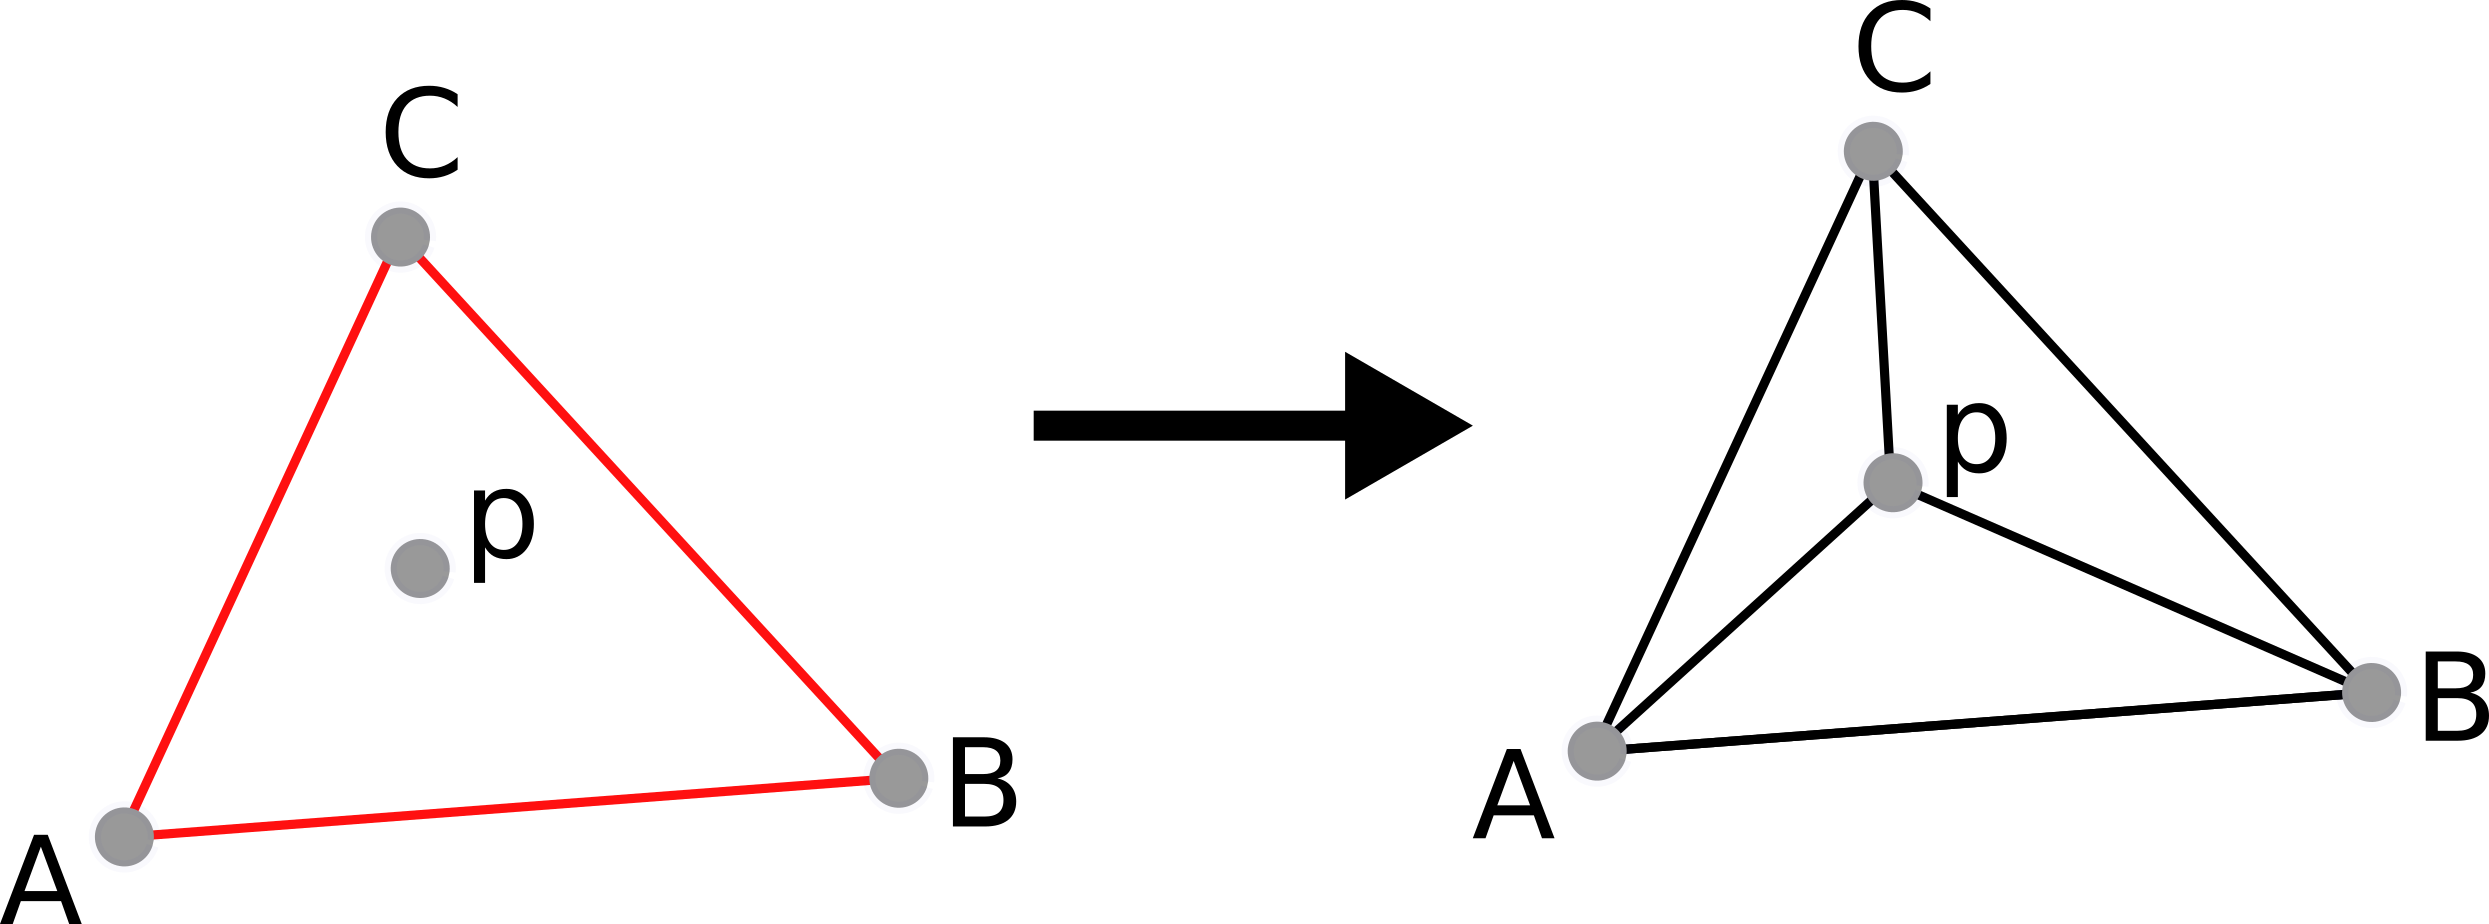
\includegraphics[scale=2]{split_triangle}
    \caption{\label{split_triangle} {\tt split\_triangle}}
\end{figure}

 The proved theorem was:\\
{\tt Theorem triangulation\_split\_triangle:\\
  $\forall$ tr, t, p, d, d != fset0 -> p $\notin$ d $\rightarrow$
                        triangulation tr d $\rightarrow$ t $\in$ tr ->\\
                        in\_triangle t p $\rightarrow$
                        triangulation (split\_triangle tr t p) (p |` d).\\
                       }
In english, this would be written as:
\begin{theorem}
  For all triangulation $tr$ of a nonempty data set $d$,
  for all triangle $t$ of this triangulation and point $p$ strictly in this triangle,
  if $p$ is not in $d$, then
  {\tt split\_triangle tr t p} is a triangulation for the data set $d \cup \{p\}$.
\end{theorem}

As one could notice, the fact that we put {\tt in\_triangle t p} and not {\tt in\_triangle\_w\_edges t p} as hypothesis means that we don't treat the case where the point we add is on the edge of a triangle, as said before. 

This theorem is proven by showing the preservation of the seven properties described in the definition of a triangulation (Section \ref{definition_triangulation}).

The proofs the preservation of the seven properties were more or less done with the same pattern: they were big case-based reasoning that also needed the proofs of some lemmas. I'll list here the most relevant ones:
\begin{enumerate}
\item If we add to the data set a point that was already in the convex hull of the data set, then the convex hull of the new data set obtained is the same.
\item A point was in the triangle $t$ deleted from the triangulation by {\tt split\_triangle}, if and only if if is in one of the new three triangles created by {\tt split\_triangle}.
\item If a point is in the interior of one of the three new triangles created by {\tt split\_triangle}, then it was in the interior of $t$.
\end{enumerate}

Even if could seem quite intuitive, the proof of the first lemma was actually quite hard to write in {\sc Coq} because of complicated problems of typings within the BigOps part of {\sc MathComp}.

The proof of the second lemma was actually very hard and long. It is a case-based reasoning on the position of the point in the big triangle. A trick was used to do the proof: I was certain that some hypotheses were not consistent (and thus I could do a proof by contradiction in some cases), but I was not able to find how to use Knuth's axioms to prove it. After a discussion with Yves Bertot, we used an automated tool made by some previous students that tested the consistency of a list of hypotheses (of the type {\tt is\_left\_of A B C} ...) using Knuth's axioms, and finally found how to finish this proof from analysing the results.

Some sommon difficulties in the proofs were due to the nature of {\sc Coq}, and how my formalisation was written : lots of times, I was left with a big case-based reasonning, with lots of case that were either absurd, or that looked a lot like previous cases but with small differences (for instance, a case with $a$ as a first vertex of a triangle and $b$ and $c$ as second and third vertices, and the case where $b$ was the first vertex, and $c$ and $a$ the second and third ones). One of the main difficulty was to try and automatise my proofs as much as possible in order to avoid aving very long proofs with lots of repeated parts.

  
\subsection{Flipping edges}
The next big step was writing the edge-flipping step (Figure \ref{flip_edge}) {\tt flip\_edge $tr$ $t1$ $t2$ $a$ $b$ $c$ $d$}.
It returns $(tr \smallsetminus t1 \smallsetminus t2) \cup \{abd;bcd\}$. It is meant to be called, in the whole algorithm, with $t1 = abc$ and $t2=acd$.

\begin{figure}
  \centering
  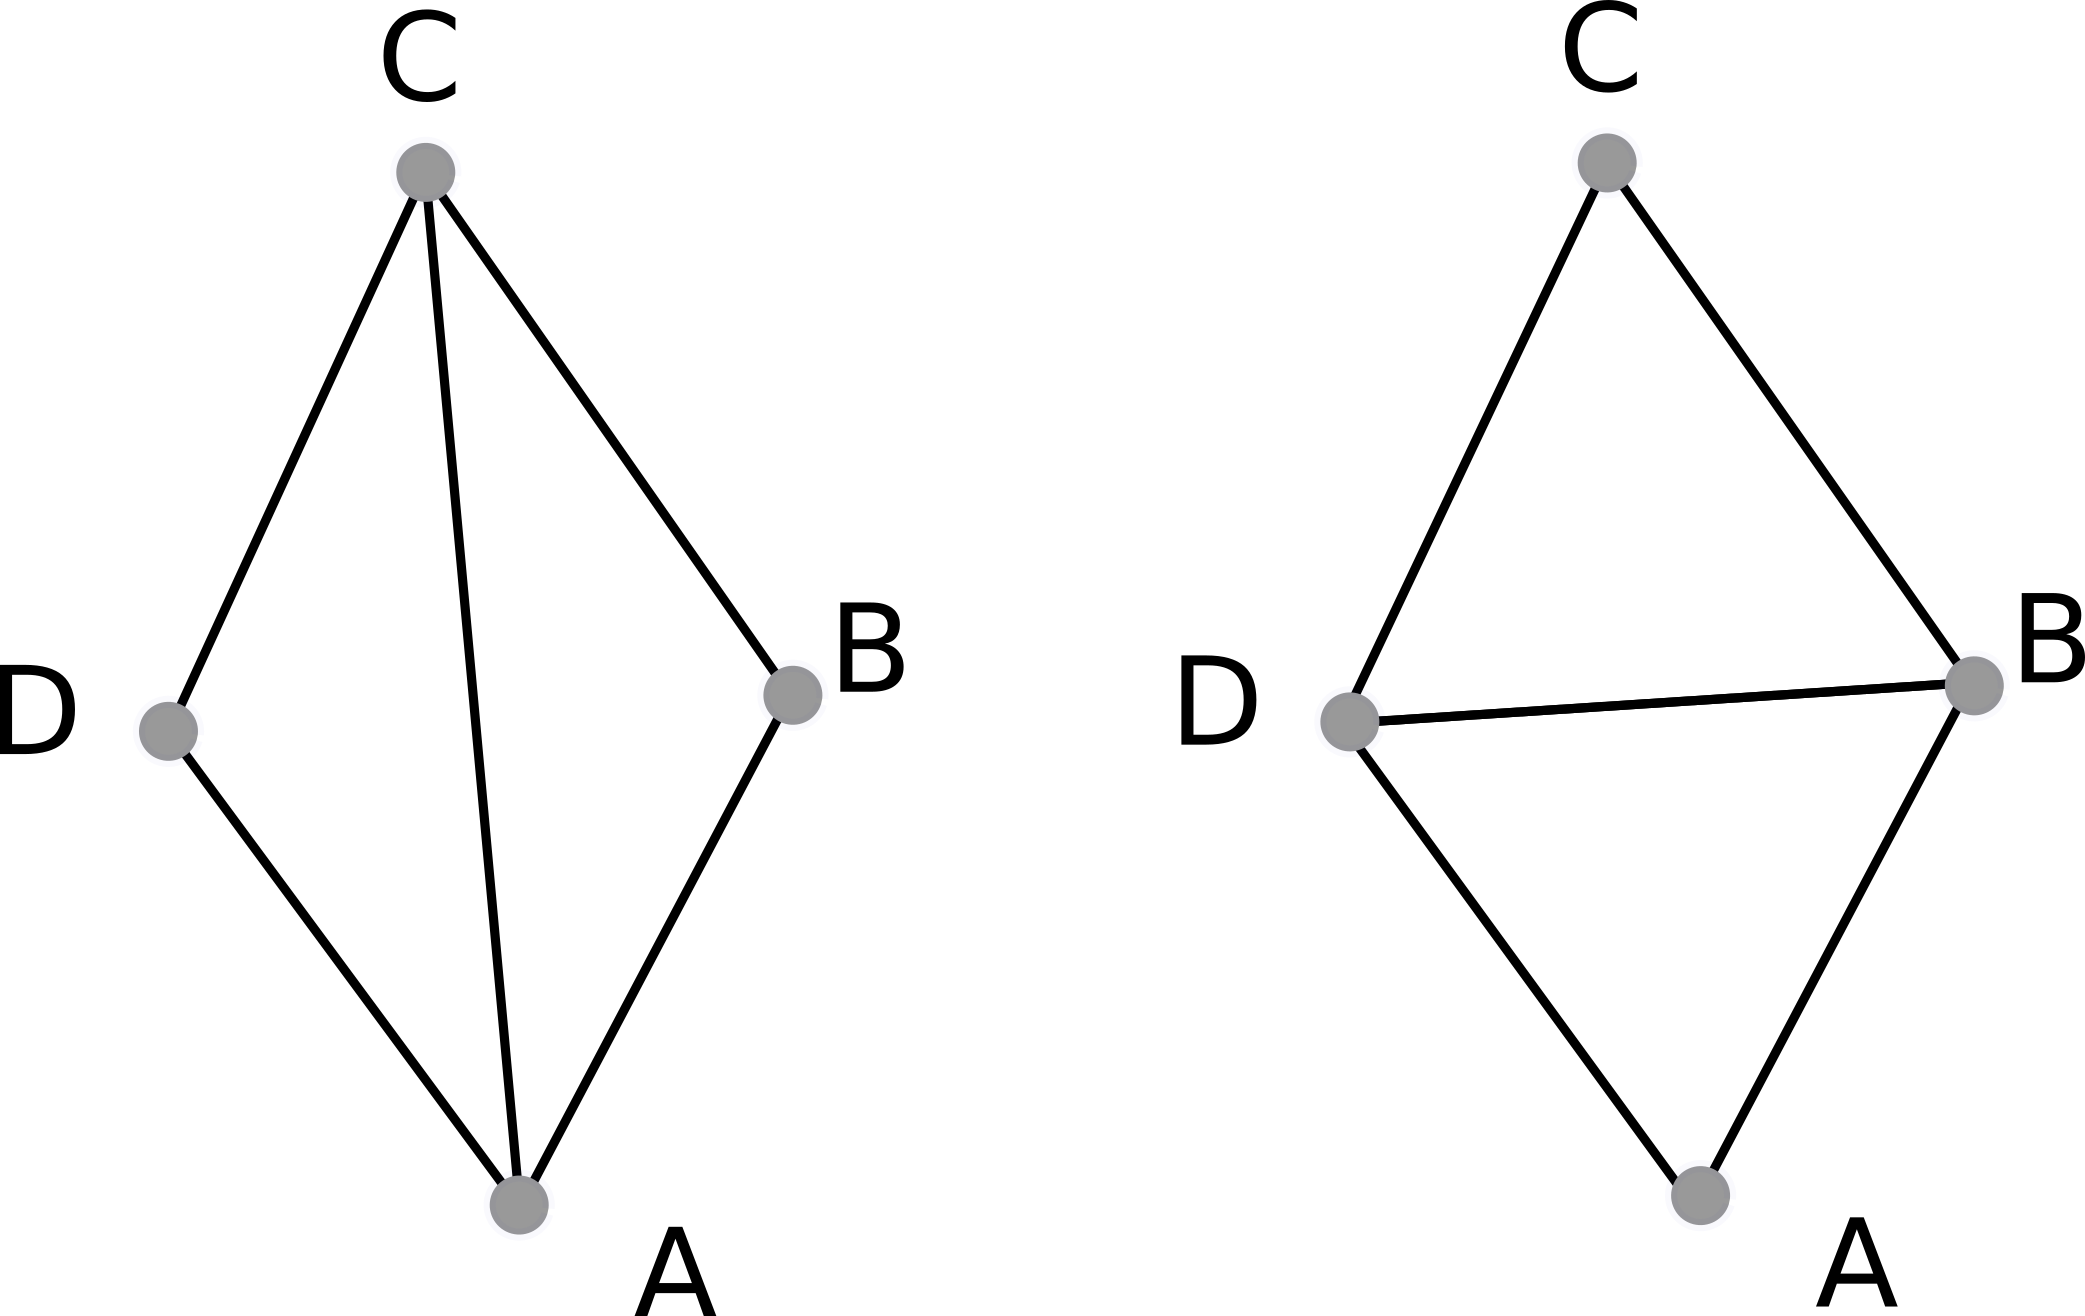
\includegraphics[scale=2]{flip_edge}
    \caption{\label{flip_edge} An edge-flipping step}
\end{figure}

I won't write here the theorem I proved, but, basically, the idea is the same as before (prove that a triangulation is transformed into another one, but with more conditions):
\begin{itemize}
\item $t_1$ and $t_2$ should be triangles of a triangulation $tr$ on a data set $D$.  
\item $a$,$b$ and $c$ should be points of the data set, vertices of $t_1$ and form a well oriented triangle (we have {\tt is\_left\_of $a$ $b$ $c$})
\item $a$,$c$ and $d$ should be points of the data set, vertices of $t_2$ and form a well oriented triangle (we have {\tt is\_left\_of $a$ $c$ $d$})
\end{itemize}
Again, this is proven by proving the preservation of the seven properties.

As before, the proofs were all big case-based reasoning that used some lemmas. Just as before, I'll try to list and explain how I proved the most relevant ones :
\begin{enumerate}
\item If a point was in one of the two triangles deleted by {\tt flip\_edge}, the it is in one of the two triangles created by {\tt flip\_edge} (see Figure \ref{flip_edge}).
\item If a point $q$ was in the interior of one of the two triangles deleted by {\tt flip\_edge}, then it if either in the interior of one of the two new triangles, or on the common edge of those triangles (this case is representated in Figure \ref{fenci}).
\item If $a,b$ and $c$ are in the vertex set of a triangle $t$, if $t$ is well oriented, then, for all $p$, $p$ is in {\tt vertices\_to\_triangle $a$ $b$ $c$} if and only if $p$ is in $t$
\end{enumerate}

\begin{figure}
  \centering
  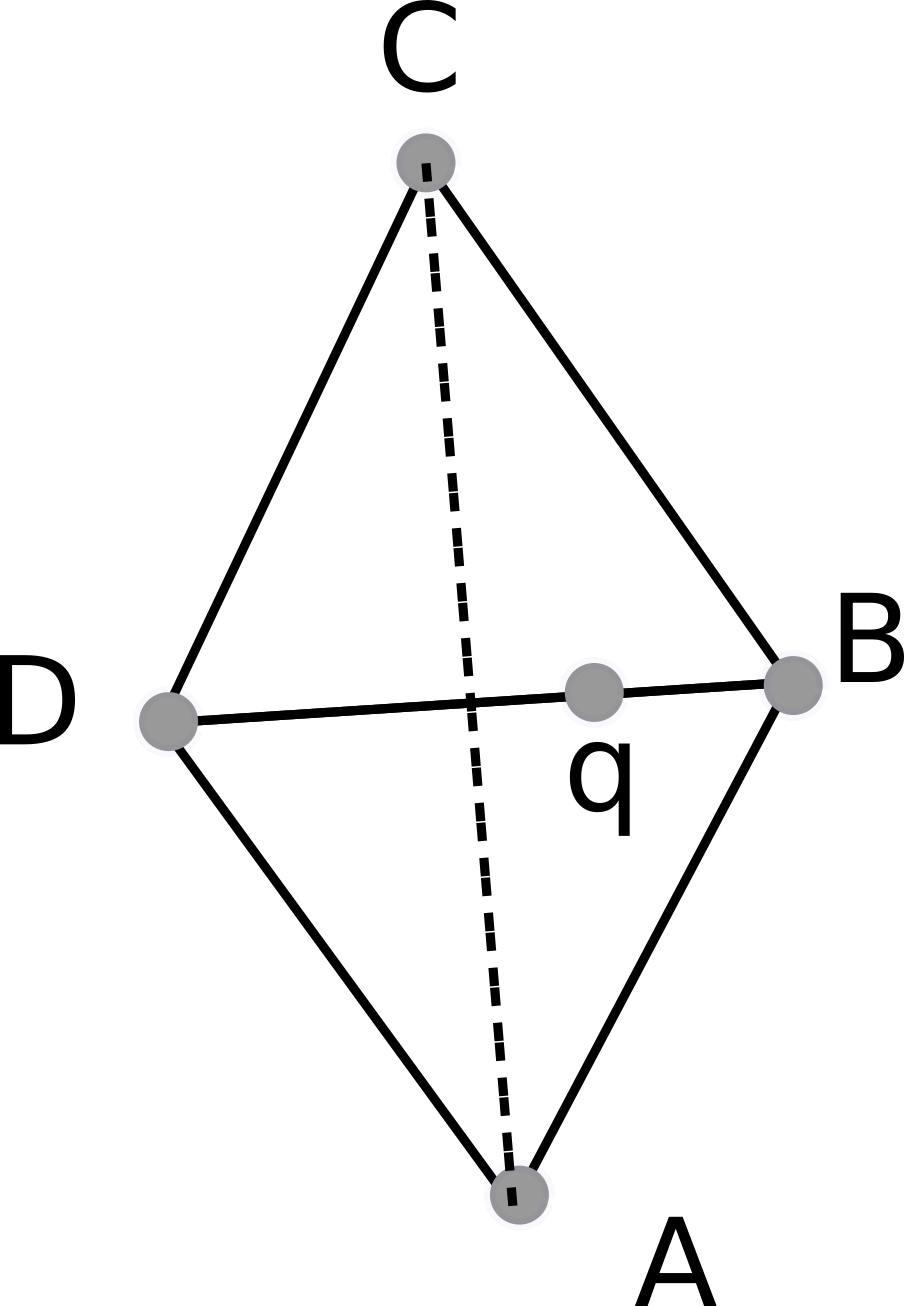
\includegraphics[scale=2]{flip_edge_nci}
    \caption{\label{fenci} Here, the point is on the common edge}
\end{figure}


The first lemma looks a lot like a previous lemma, already proven for {\tt split\_triangle}. Its proof is already a lot alike. However, thank to the experience I gained proving other lemmas inbetween, I managed to to a way better proof (it is better automated and thus shorter).

The third lemma looks very simple to prove since {\tt vertices\_to\_triangle} always return oriented triangles by hypothesis. However, this proof wasn't actually simple, and made me realize that a theorem was missing in Cyril Cohen's Finmap library \cite{finmap}, which was quickly added with his help.

\subsection{Remarks}

Proving the preservation of these properties was the main part of the internship. While they looked very simple to prove by hand, proving them in {\sc Coq} was a way more difficult task.

Indeed, {\sc Coq} prevents us from using the mental shortcuts that we use unconsciously to shorten proofs (and it is actually a good aspect about {\sc Coq}, because mental shortcuts can induce false proofs on paper, because we often forgent degenerate cases or hypotheses). One of the most important thing to remember, when proving theorems with {\sc Coq} and the {\sc Mathematical Component} library, is that it is usually best to try and make a plan for the proof, on paper, and then try to follow this plan.  If something is wrong during the proof and it becomes no longer possible to follow the plan, it is that either there is a problem with the proof, or that there is something missing in the library. It is actually very easy to get trapped by {\sc Coq} and try to do the proof by following {\sc Coq} instead of a proof plan!

\section{Instantiation of the model}
\rule{\linewidth}{0.5pt}
\label{implementation}
The next step of the work was to do an instantiation of the model (choices for the implementation of the types like {\tt P} and functions like {\tt vertices\_to\_triangle}. For the types:
\begin{itemize}
\item A point is a vector of size 2 of reals: \definition{P}{$'rV[R]_2$. }
\item A triangle is a vector of size 3 of points: \definition{T}{$'rV[P]_3$. }
\item An edge is a vector of size 2 of points: \definition{E}{$'rV[P]_2$. }
\end{itemize}
For the implementation of the functions, with ord$nx$ being the $(x+1)^{\text{th}}$ element of the set containing the elements of $\mathbb{N}$ inferior to n).
 \begin{itemize}
  \item \definition{xCoord (p: P)}{p ord10 ord20} \\(in {\sc MathComp}, a vector of elements of $\mathbb{R}$ of size 2 is a function from the Ordinal 1 to the Ordinal 2 in $\mathbb{R}$). 
  \item \definition{yCoord (p: P)}{p ord10 ord21}.
   \item \definition{vertex (t: T)}{t ord10} which gives a function from the Ordinal 3 to P.
\item {\tt oriented\_surface a b c} \label{oriented_surface} can be defined as the determinant of the matrix:
  $$ \left( \begin{matrix}
1 & \text{{\tt xCoord  a}} & \text{{\tt yCoord  a}}\\
1 & \text{{\tt xCoord  b}} & \text{{\tt yCoord  b}}\\
1 & \text{{\tt xCoord  c}} & \text{{\tt yCoord  c}}
\end{matrix} \right) $$\\
This way, most proofs on {\tt oriented\_surface} are very nice to do: one only needs to expand the determinant and then use automatic tactics on rings. The only difficulty was to add the ring on which we worked ($\mathbb{R}$ with the usual operations) so that the automatic tactic {\tt ring} worked (the tactic {\tt ring} works by having a set of usual rings on which it knows how to do operations, what lemma to use for transitivity and other properties of the operations, etc).

\item The predicate {\tt in\_circle p a b c}, testing if p is in the circumcircle of the triangle {\tt abc}, can also be defined as testing if the determinant of the following matrix is nonpositive:

  $$\left( \begin{matrix}
1 & \text{{\tt xCoord  p}} & \text{{\tt yCoord  p}}& \text{{\tt (xCoord  p)$^2$ + (yCoord  p)$^2$}}\\
1 & \text{{\tt xCoord  a}} & \text{{\tt yCoord  a}}& \text{{\tt (xCoord  a)$^2$ + (yCoord  a)$^2$}}\\
1 & \text{{\tt xCoord  b}} & \text{{\tt yCoord  b}}& \text{{\tt (xCoord  b)$^2$ + (yCoord  b)$^2$}}\\
1 & \text{{\tt xCoord  c}} & \text{{\tt yCoord  c}}& \text{{\tt (xCoord  c)$^2$ + (yCoord  c)$^2$}}
\end{matrix} \right) $$\\
\item The implementations of {\tt vertices\_to\_triangle} and {\tt vertices\_to\_edge} were not direct to write.

  First, for {\tt vertices\_to\_triangle a b c}, since we require in the formalisation that any triangle obtained by {\tt vertices\_to\_triangle} should be well-oriented, we have to check if $abc$s form a well-oriented triangle. If it does, we return $abc$; otherwise, we return $bac$ which will be oriented by definition of the {\tt is\_left\_of} predicate.

  Then, for {\tt vertices\_to\_edge}, we require, for every {\tt a} and {\tt b}, that {\tt vertices\_to\_edge a b } = {\tt vertices\_to\_edge b a}. To ensure this property, we define a lexicographic order on points. Then, if {\tt a} $\leq$ {\tt b}, we return {\tt ab}; otherwise, we return {\tt ba}.
\end{itemize}
The proofs can be grouped in several types:
\begin{itemize}
\item The proofs on geometrical predicates (for instance, the fact that {\tt oriented\_surface a b c} = {\tt oriented\_surface b c a} = {- \tt oriented\_surface b a c}) were quite easy because of the fact that proofs on determinants only require to expand the determinants and then do some calculus, which is automatic with the tactic {\tt ring}. I reused some work done by a previous intern, Wassim Haffaf, in this part (the way he expanded 3 x 3 determinants for instance).
\item The proofs requiring more geometrical work (a good example of this is the proof of the hypothesis {\tt on\_edge\_on\_line}, see Section \ref{Hypothesis}).

  Those were way harder and I didn't have the time to finish them all. {\tt on\_edge\_on\_line} and {\tt on\_line\_on\_edge} are two examples of proofs that I tried to do but couldn't finish since they were very challenging and I was running out of time.
  \item The proofs on the functions (for instance, the proofs on {\tt edges\_set} and {\tt vertices\_to\_triangle}). Those were generally simpler than the previous type of proofs (the difficulty coming more from the use of {\sc Coq} and how to do case-based reasoning in an intelligent/automatic way, more than from geometrical problems). I still couldn't finish them all, but I managed to complete a good part of them. 

  \item The proofs of Knuth's axioms.

    I didn't have time to begin proving these at all. However, a number of them could probably be recovered from previous work done by other students (for instance, the work on convex hulls done by David Pichardie (see \cite{Hull}).
  \end{itemize}

  The instantiation of the model was a very interesting part of the internship. When I tried to do it, I realised a lot of problems about the first version of my formalisation of Delaunay triangulations: some hypotheses were not precise enough, some were even false. For instance, I realised that, often, it was hard for me to keep in mind that triangles can be flat when thinking about the correctness of some hypotheses. Thus, I had to rewrite a lot of hypotheses and proofs.


%\section{Examples of proofs}
%\rule{\linewidth}{0.5pt}
%\label{example}
%\label{easygeo}*)
\newpage
\section{Conclusion}
\rule{\linewidth}{0.5pt}
The goal of this internship was formalising the concept of Delaunay triangulation in {\sc Coq}, expressing a classic incremental algorithm to compute them and proving its correctness. During the time I had, I managed to :
\begin{enumerate}
\item write the formalisation and an implementation of this formalisation;
\item prove a part of the hypotheses and some useful lemmas;
\item write the two steps of the algorithm (but not the algorithm itself);
\item prove the correctness of the two steps (the fact they return a correct triangulation).
\end{enumerate}

There are some clear possible paths of improvement for my work. First, not all proofs are completed. Then, the next step for me would have been to implement the whole algorithm itself in {\sc Coq}, from the different steps ({\tt split\_ttriangle} and {\tt flip\_edge}) I wrote. The biggest difficulty would have been to prove the termination of the algorithm which transform a random triangulation into a Delaunay triangulation: the way it is done is by noticing that, during execution of the algorithm, the lifted image of the triangulation on the unit paraboloid is a quantity that is decreasing \footnote{A more detailed explanation of this possible proof can be found here:
\href{https://www.ti.inf.ethz.ch/ew/Lehre/CG13/lecture/Chapter 6.pdf}{https://www.ti.inf.ethz.ch/ew/Lehre/CG13/lecture/Chapter 6.pdf}}.

Then, when this is finished, there are some other possibilities to extend my work:
\begin{enumerate}
\item First, one could generalize the formalisation of Delaunay triangulations to algorithms that work in higher dimension. In fact, the method I formalised, that is the incremental construction using flips, can be generalized in dimension 3 or higher \cite{CompGeoAlgo}. However, the complexity is exponential in the dimension (as shown in \cite{IncrementalDimension})
\item Another idea could be to try and formalise other Delaunay triangulation algorithm. It is shown in \cite{Comparison} that the most efficient method to compute Delaunay Triangulation is a Divide and Conquer algorithm presented in \cite{AlgoDivide}. An implementation of this algorithm is presented here:\\
  \href{http://www.geom.uiuc.edu/~samuelp/del_project.html}{{\tt http://www.geom.uiuc.edu/$\sim$samuelp/del\_project.html}}
\end{enumerate}

There are also some things that could be changed about the work I have done.

First, my proficiency with {\sc Coq} and, especially, {\sc SSReflect}, changed during the internship. I already followed, before this, a one-week course on {\sc SSReflect} and I did an internship in IRISA Rennes where I used {\sc Coq} to do proofs on programs. However, this was not comparable to how I had to use {\sc Coq} during this internship. As such, at the beginning of this internship, I took a lot of time to prove results that would have been way easier for me at the end of the internship.

  Moreover, the proofs I wrote at the end of the internship are better written than the one I have done at the beginning at the internship, taking advantage from the use of the syntax of {\tt SSReflect} and of tricks such as the use of the tactic {\tt try}.

\section{Acknowledgements}
I would like to thank a lot my supervisor, Yves Bertot for all the time he spent helping me during this internship, and all the good references he gave me. I would also like to acknowledge Cyril Cohen, who helped me a lot during the internship, as well asz Laurence Rideau, who helped me find this internship. I also want to thank all the other members of the Marelle team at INRIA Sophia-Antipolis for their friendly welcome and help.

I would also like to acknowledge Pierre Alliez, from the TITANE team at INRIA Sophia-Antipolis for the nice and helpful discussion he granted us, which conforted us in the direction we were taking in this research.

Finally, I would like to thank Damien Rouhling from the Marelle team and Jean-Yves Franceschi from ENS Lyon for the help given, and the great advices they gave me regarding the writing of this report.

\newpage
\bibliographystyle{alpha}
\bibliography{Report}
\end{document}



